\documentclass[11pt]{article}
\usepackage[margin=1in]{geometry}

\usepackage{graphicx}
\usepackage{float}
\setlength{\textfloatsep}{10pt}

\usepackage{caption}
\captionsetup{skip=4pt}
\captionsetup{font=small}

\usepackage{placeins}

% --- Float placement relaxation to reduce white space ---
\renewcommand{\topfraction}{0.9}
\renewcommand{\bottomfraction}{0.8}
\renewcommand{\textfraction}{0.1}
\renewcommand{\floatpagefraction}{0.85}

\title{Analysis of Cable Thickness Effects on Capacitance Readings}
\author{Mani}
\date{\today}

\begin{document}
	
	\begin{titlepage}
		\centering
		{\Huge Analysis of Cable Thickness Effects on Capacitance Readings\par}
		
		\vspace{1cm}
		
		{\large Mani Asadiasadabad\par}
		
		\vfill
		
		University of South Carolina
		
		\today
	\end{titlepage}
	\newpage
	
	\begin{center}
		{\Large\bfseries Abstract\par}
	\end{center}
	
	\noindent
	The objective of this experiment was to evaluate the effect of cable thickness on capacitance measurements and to see which cable provides the cleanest and most accurate data. Three different cables with conductor diameters of approximately 0.64 mm, 0.40 mm, and 0.32 mm were tested under stationary and moving conditions. A DAQ was used for capacitance readings and the data were processed, filtered, and analyzed using MATLAB. Frequency-domain analysis was also performed using the Fast Fourier Transform (FFT). The thinnest (0.32 mm) and the medium-thickness (0.40 mm) cables performed almost identically during the stationary testing, both collecting cleaner and less noisy data compared to the thickest cable (0.64 mm). For the moving condition, however, the thinnest cable performed slightly better than the medium cable, with both collecting significantly more accurate capacitance readings consistently. These results indicate that cable conductor size influences signal quality and should be considered when selecting instrumentation for capacitance measurements.
	
	\section{Introduction}
	
	Capacitance-based sensing systems are widely used for detecting changes in physical properties because they provide high sensitivity. Accurate signal acquisition depends not only on the capacitive sensor, but also on the quality and thickness of the cable used to collect the data. Signal distortion caused by cable selection can introduce noise and reduce measurement accuracy. Understanding how cables affect these readings can help us reduce noise as much as possible and collect reliable data.
	
	This report investigates the effect of triaxial cable thickness (conductor diameter) on capacitance measurements. Three cables with different thicknesses were tested under both stationary and moving conditions. The main objective of this experiment was to determine how cable thickness affects capacitance data collection and to identify the cable that provides the most accurate and least noisy capacitance readings.
	
	\section{Experimental Setup}
	
	For this experiment, three triaxial cables with approximate conductor diameters of 0.64 mm (\textbf{22 AWG}), 0.40 mm (\textbf{RG-174}), and 0.32 mm (\textbf{28 AWG}) were used. A \textbf{40 pF} ceramic capacitor was soldered to each cable after the insulation was stripped from the conductor. The opposite side of each triaxial cable was soldered to a \textbf{9-pin D-sub (DE-9)} male connector. The cable's center conductor and shield (ground) were soldered to the designated pins to interface with the data acquisition (DAQ) system.
	
	To ensure consistency between tests, the same 40 pF ceramic capacitor was desoldered and transferred between the three cables, one cable at a time. Each cable was evaluated under both stationary and moving conditions, with three trials conducted for each condition. During the stationary tests, the cables were suspended from the edge of a table and remained motionless throughout each trial. During the moving tests, the cables were manually moved, bent, and vibrated at various locations, with particular emphasis on the region near the DE-9 connector. The data were collected in \textbf{LVM (LabVIEW)} format, later converted to CSV, processed, and plotted using MATLAB. The resulting data were then transformed into the frequency domain using the Fast Fourier Transform (FFT) to analyze the noise introduced by each cable at different frequencies.
	
	\section{Results}
	
	Capacitance measurements were first evaluated under stationary conditions. Three trials were performed for each cable to ensure data consistency. The filtered capacitance signals for each cable under stationary conditions are provided in Figures~\ref{fig:still-f-032}--\ref{fig:still-f-064} in the Appendix, and the individual FFT plots for each cable are shown in Figures~\ref{fig:still-c-032}--\ref{fig:still-c-064}. A direct comparison of the FFT spectra for all three cables under stationary conditions is shown in Figure~\ref{fig:still123} below.
	
	\begin{figure}[htbp]
		\centering
		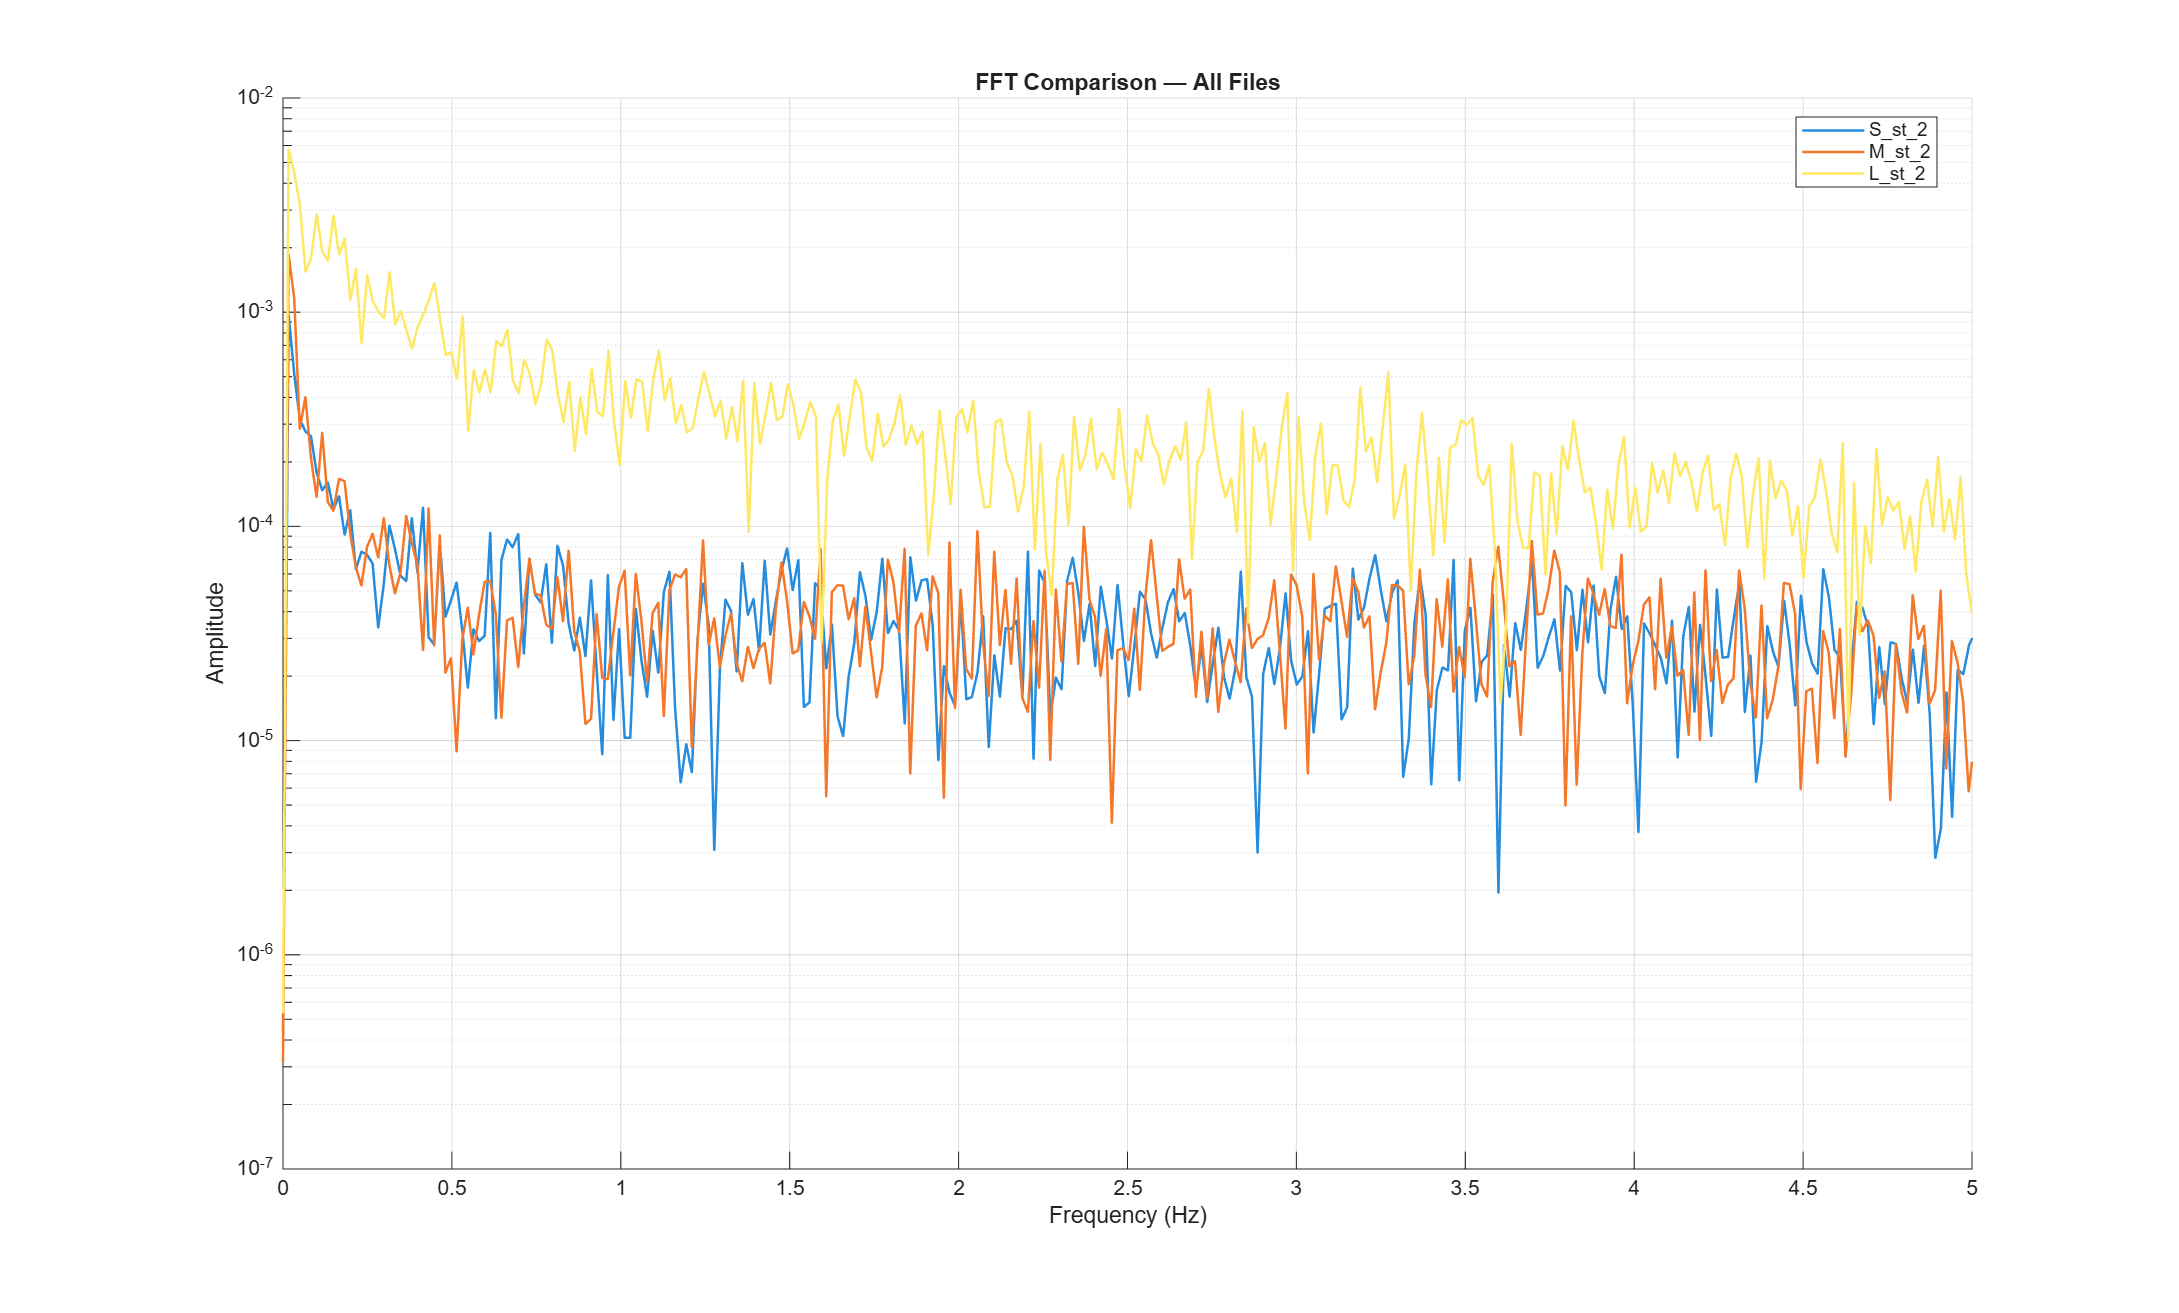
\includegraphics[width=\textwidth,height=7cm]{Figures/123_Still_Comparison.png}
		\caption{FFT comparison of all three cables under stationary conditions. The legend labels correspond to the 28 AWG (S), RG-174 (M), and 22 AWG (L) cables.}
		\label{fig:still123}
	\end{figure}
	
	Sensor capacitance was then collected under moving conditions. Three trials were conducted for each cable to ensure data consistency. The filtered capacitance signals for each cable under moving conditions are provided in Figures~\ref{fig:moving-f-032}--\ref{fig:moving-f-064} in the Appendix, and the individual FFT plots for each cable are shown in Figures~\ref{fig:moving-c-032}--\ref{fig:moving-c-064}. A direct comparison of the FFT spectra for all three cables under moving conditions is shown in Figure~\ref{fig:moving123} below.
	
	\begin{figure}[htbp]
		\centering
		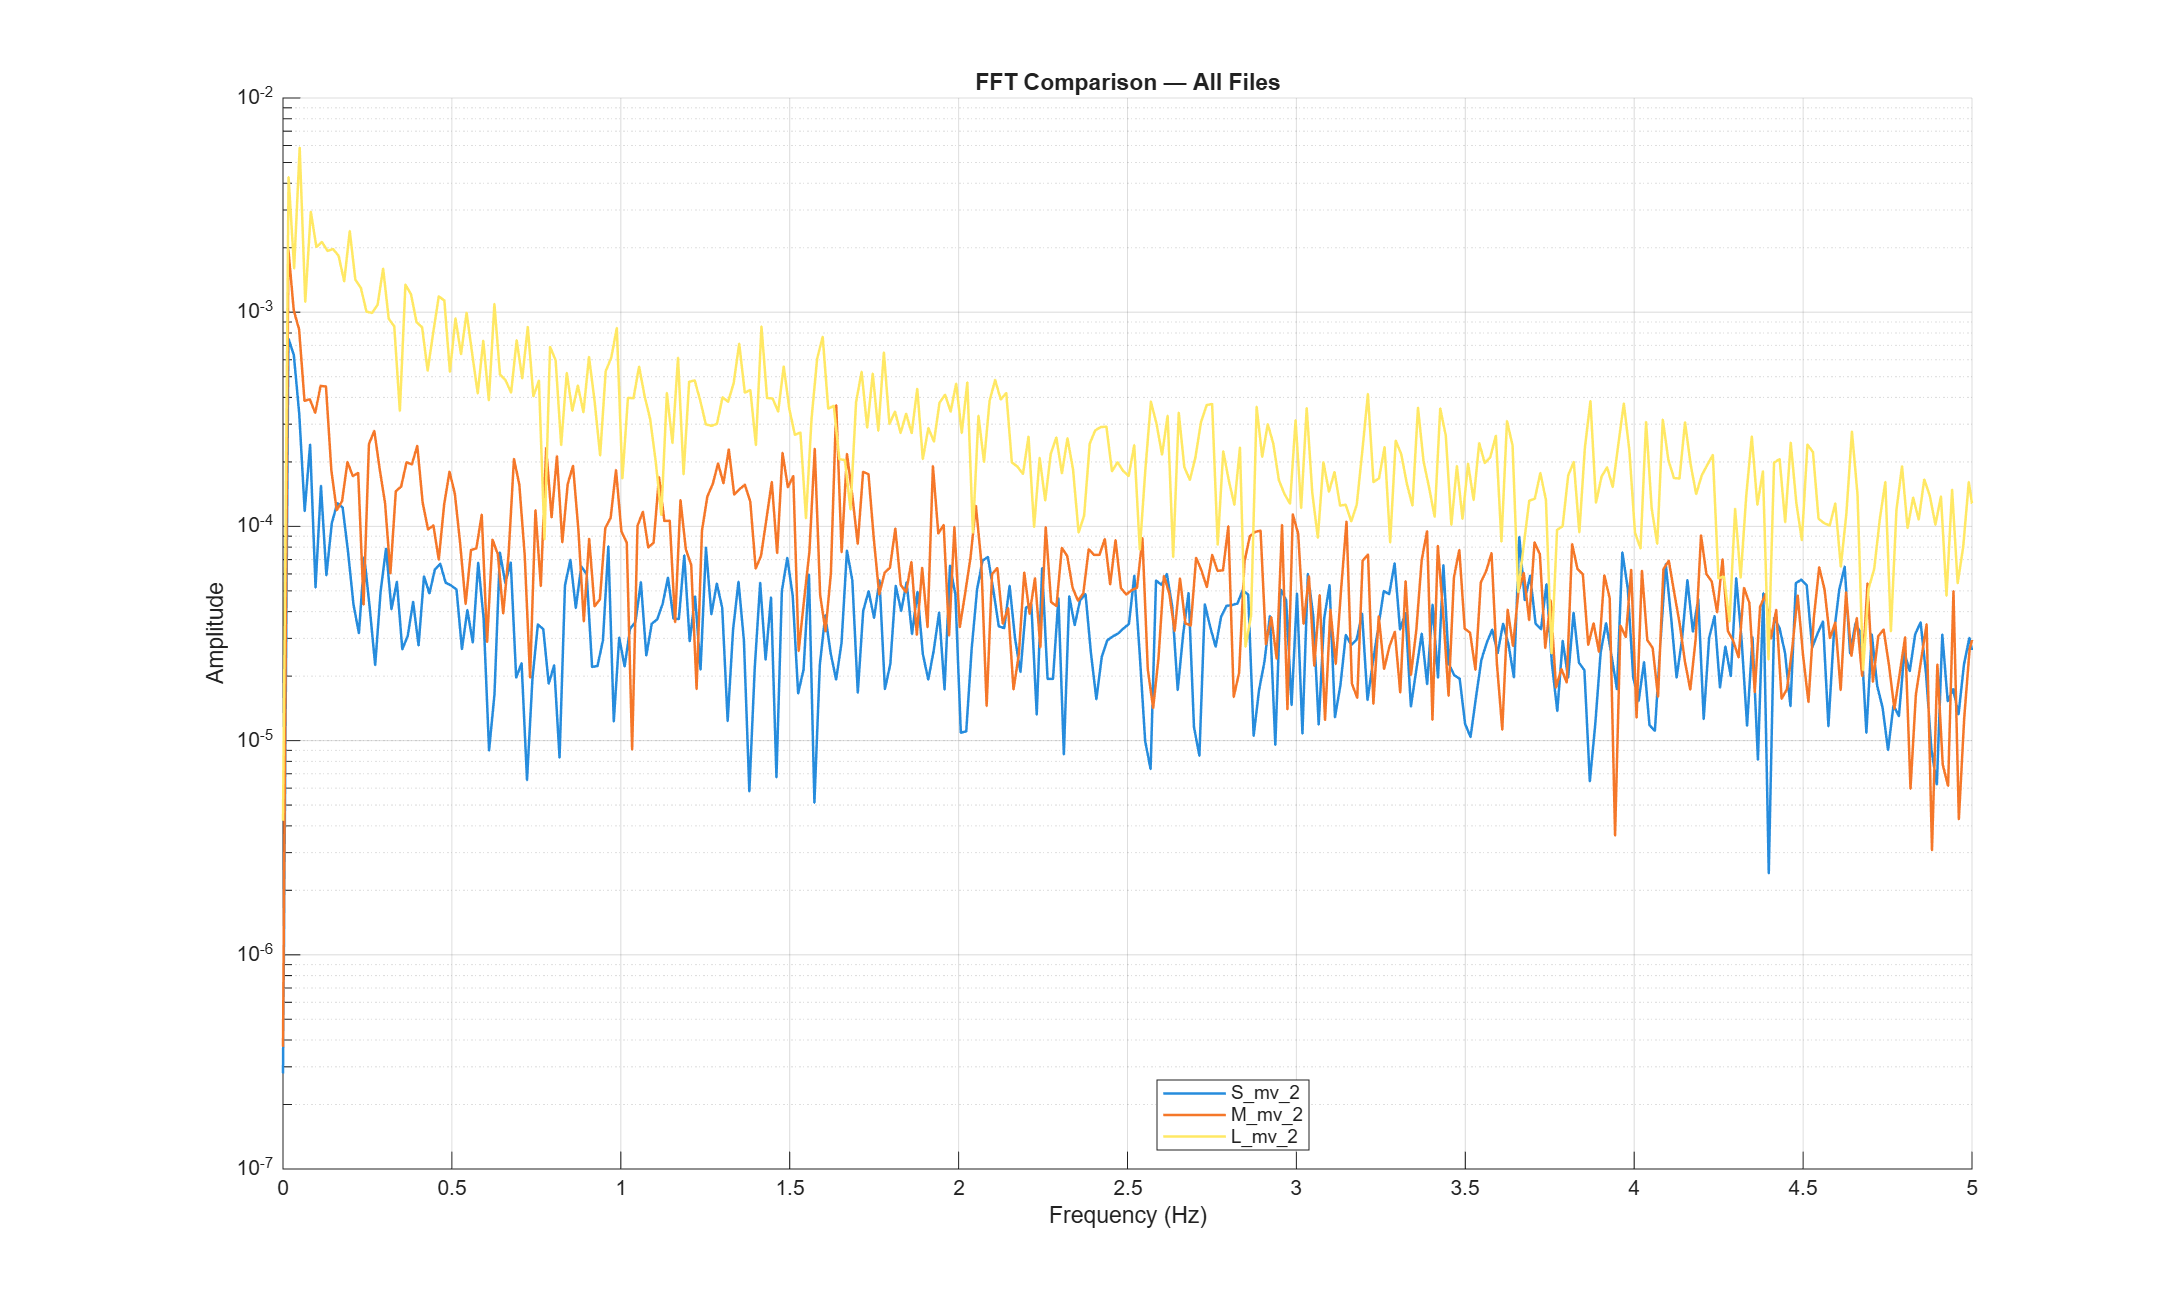
\includegraphics[width=\textwidth,height=7cm]{Figures/123_Moving_Comparison.png}
		\caption{FFT comparison of all three cables under moving conditions. The legend labels correspond to the 28 AWG (S), RG-174 (M), and 22 AWG (L) cables.}
		\label{fig:moving123}
	\end{figure}
	
	\FloatBarrier
	
	\section{Discussion}
	
	The FFT analysis indicates that the 0.64 mm (22 AWG) cable consistently exhibited the highest noise levels under both stationary and moving conditions. The 0.32 mm (28 AWG) and 0.40 mm (RG-174) cables produced substantially lower FFT amplitudes, indicating reduced frequency-domain noise. Under the stationary condition, the 0.32 mm and 0.40 mm cables performed almost identically. Under moving conditions, however, the 0.32 mm cable generally exhibited slightly lower FFT amplitudes than the 0.40 mm cable, although the difference between the two was relatively small.
	
	\vspace{0.25cm}
	
	These findings suggest that cable selection has a measurable impact on the quality of capacitance measurements. Although the 0.32 mm and 0.40 mm cables both demonstrated low noise levels, the 0.32 mm cable consistently provided the lowest overall frequency-domain response, particularly during the moving tests. In contrast, the 0.64 mm cable exhibited noticeably higher noise throughout the frequency range, indicating reduced signal quality under the tested conditions.
	
	\section{Conclusion}
	
	The objective of this study was to evaluate the effect of cable thickness on capacitance measurements. Based on the time-domain and frequency-domain analyses, the 0.32 mm cable demonstrated the best overall performance, while the 0.64 mm cable consistently exhibited the highest noise levels. These results indicate that cable selection plays an important role in obtaining reliable capacitance measurements and should be considered when designing future measurement systems.
	
	\clearpage
	\appendix
	\section{Supplementary Figures}
	
	This appendix contains the individual filtered capacitance signals and FFT plots for each cable configuration, referenced in Section~3.
	
	\subsection{Stationary Conditions}
	
	\vspace{1cm}
	
	\begin{figure}[htbp]
		\centering
		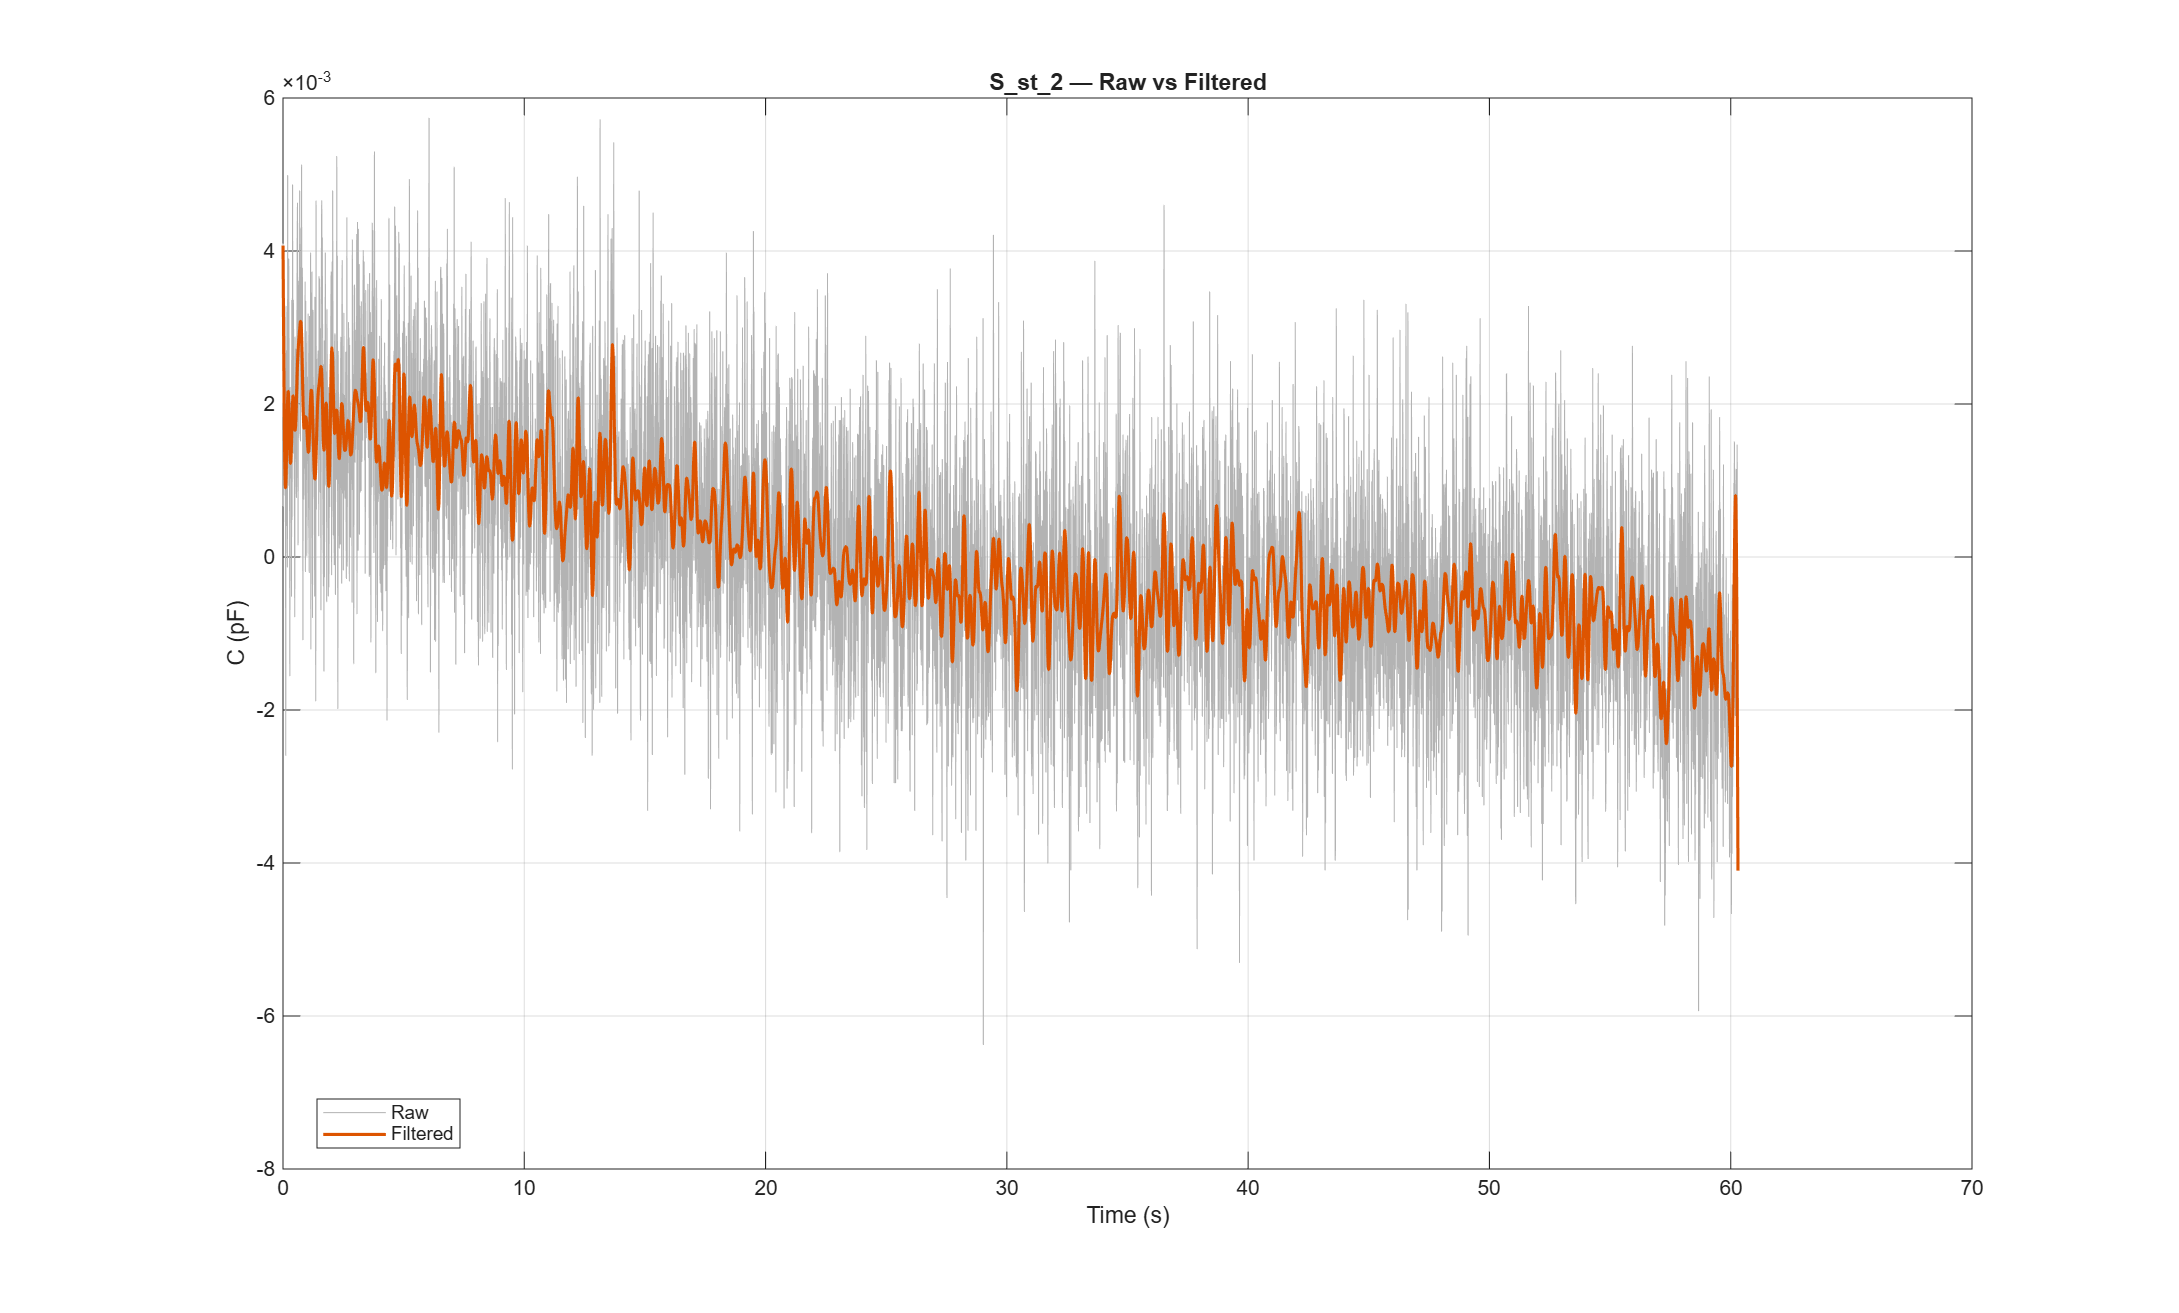
\includegraphics[width=\textwidth,height=7cm]{Figures/1_Still_filtered.png}
		\caption{Filtered capacitance measurements for the 0.32 mm cable under stationary conditions.}
		\label{fig:still-f-032}
	\end{figure}
	
	\vspace{1cm}
	
	\begin{figure}[htbp]
		\centering
		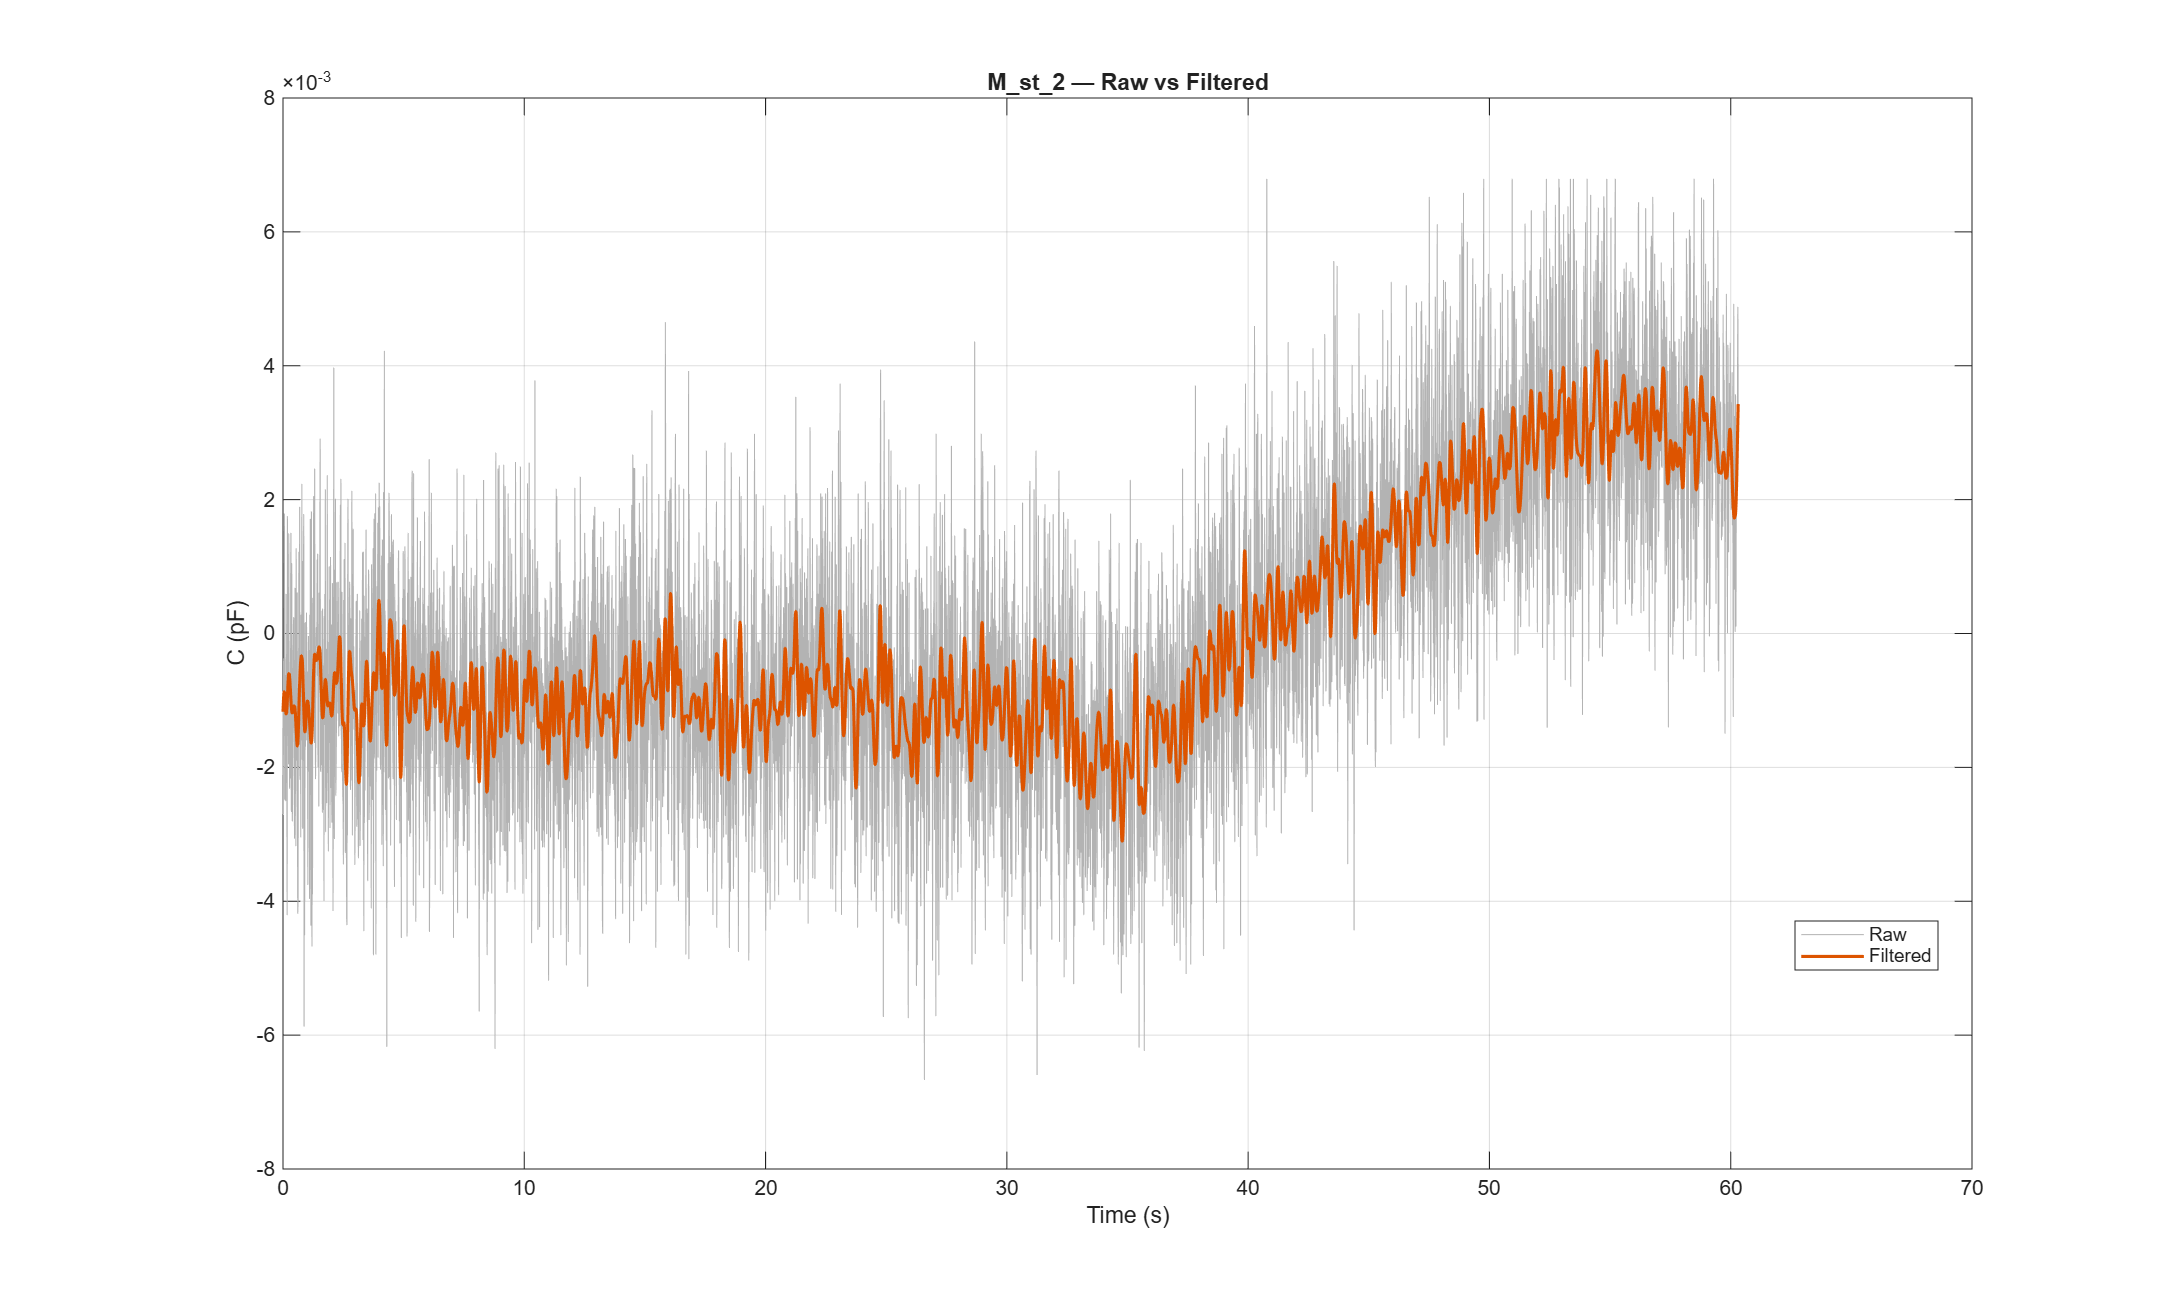
\includegraphics[width=\textwidth,height=7cm]{Figures/2_Still_filtered.png}
		\caption{Filtered capacitance measurements for the 0.40 mm cable under stationary conditions.}
		\label{fig:still-f-040}
	\end{figure}
	
	\begin{figure}[htbp]
		\centering
		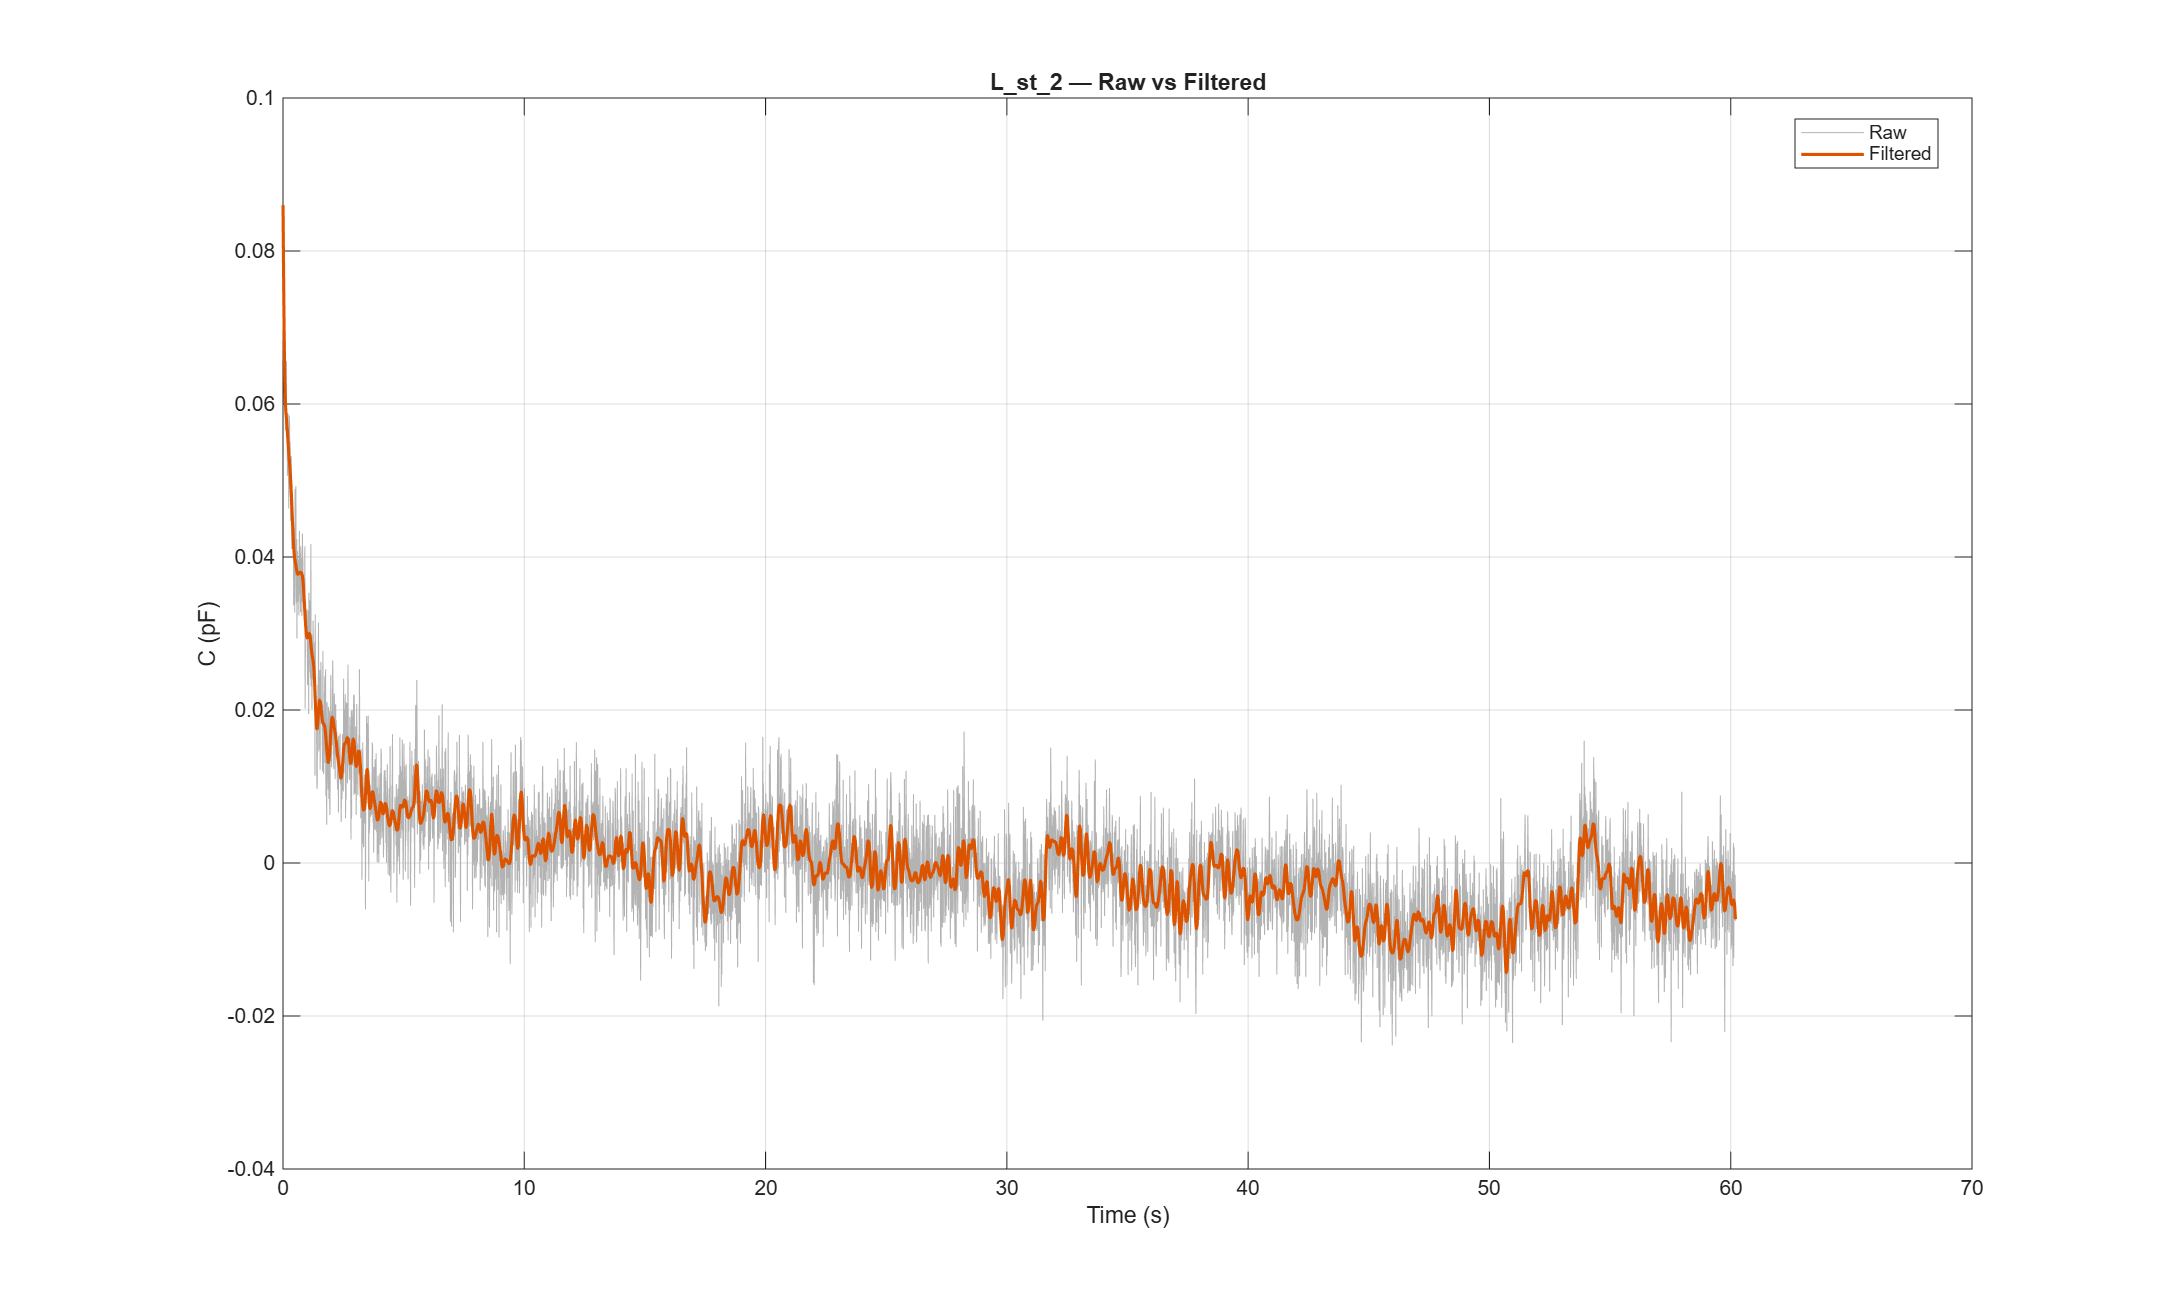
\includegraphics[width=\textwidth,height=7cm]{Figures/3_Still_filtered.png}
		\caption{Filtered capacitance measurements for the 0.64 mm cable under stationary conditions.}
		\label{fig:still-f-064}
	\end{figure}
	
	\begin{figure}[htbp]
		\centering
		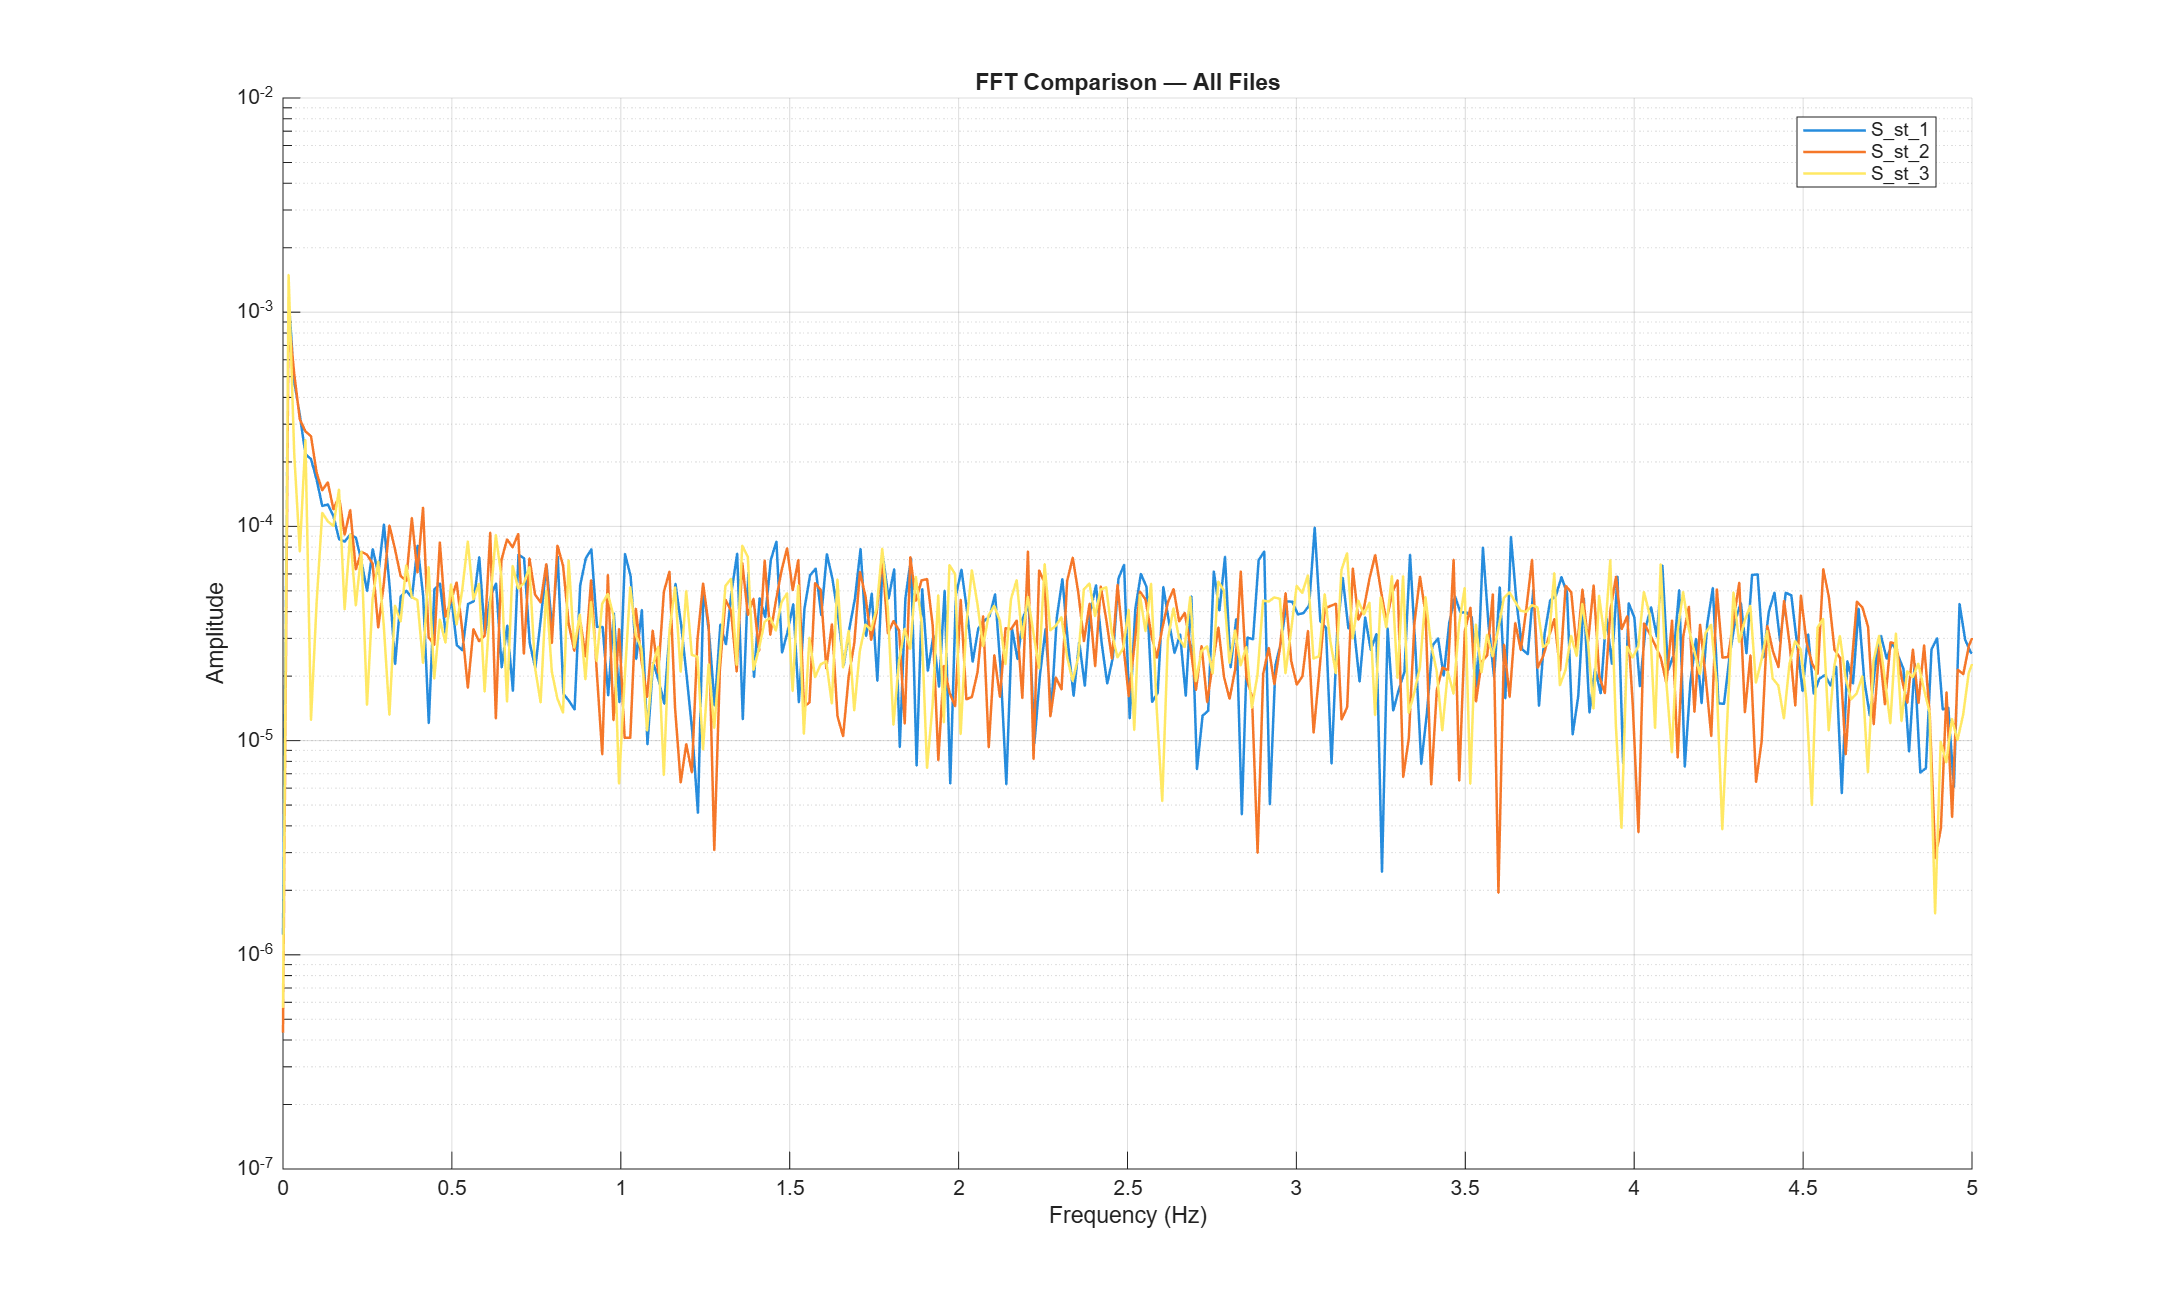
\includegraphics[width=\textwidth,height=7cm]{Figures/1_Still_Comparison.png}
		\caption{FFT plot for the 0.32 mm cable under stationary conditions.}
		\label{fig:still-c-032}
	\end{figure}
	
	\begin{figure}[htbp]
		\centering
		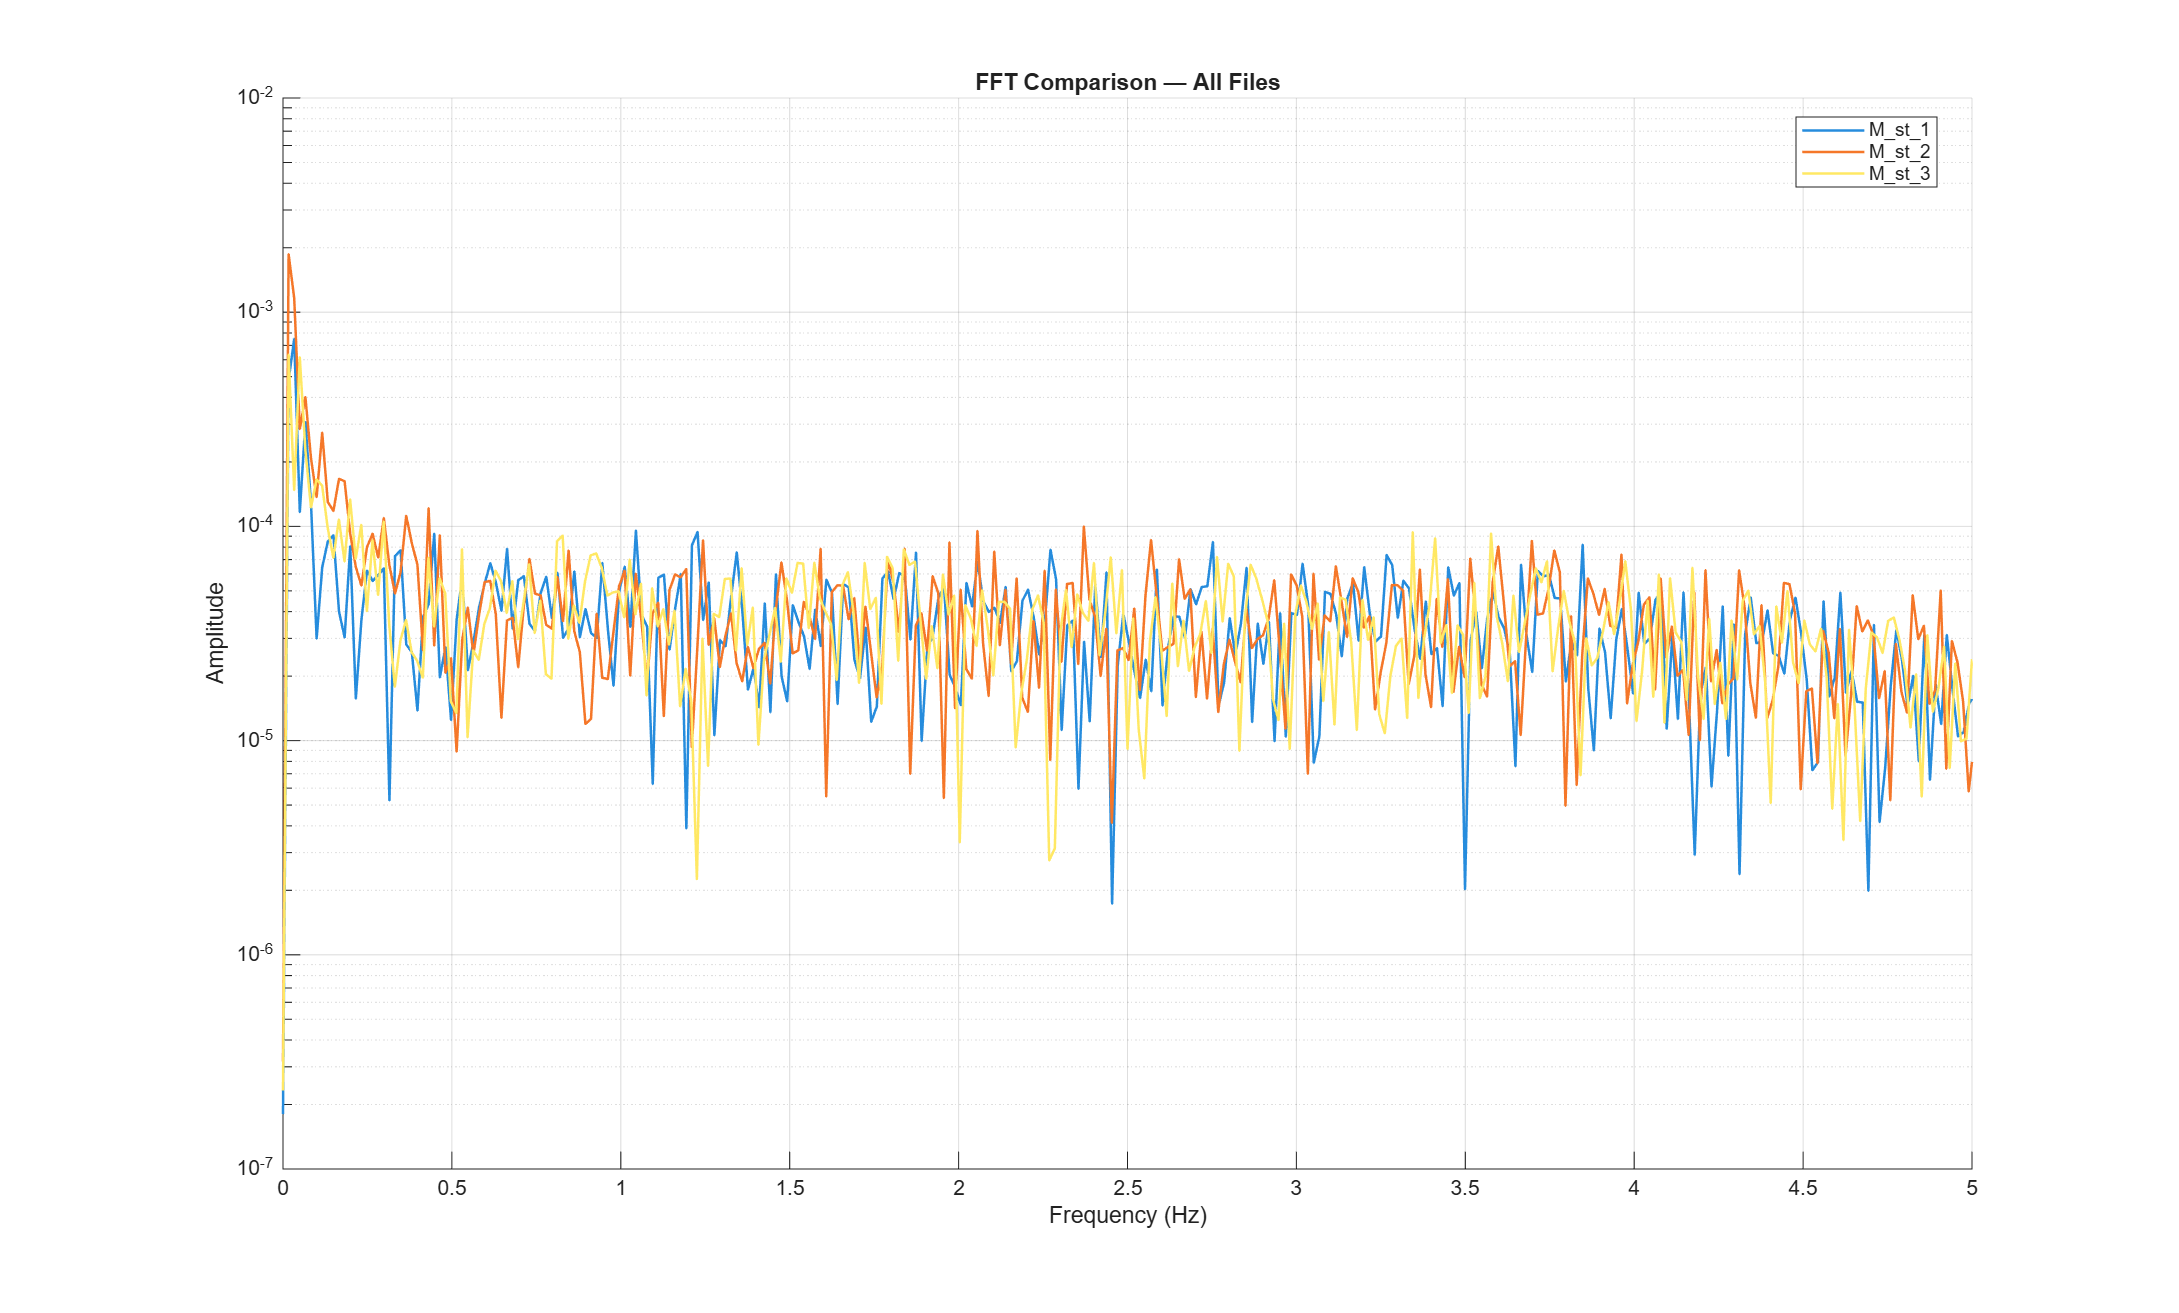
\includegraphics[width=\textwidth,height=7cm]{Figures/2_Still_Comparison.png}
		\caption{FFT plot for the 0.40 mm cable under stationary conditions.}
		\label{fig:still-c-040}
	\end{figure}
	
	\begin{figure}[htbp]
		\centering
		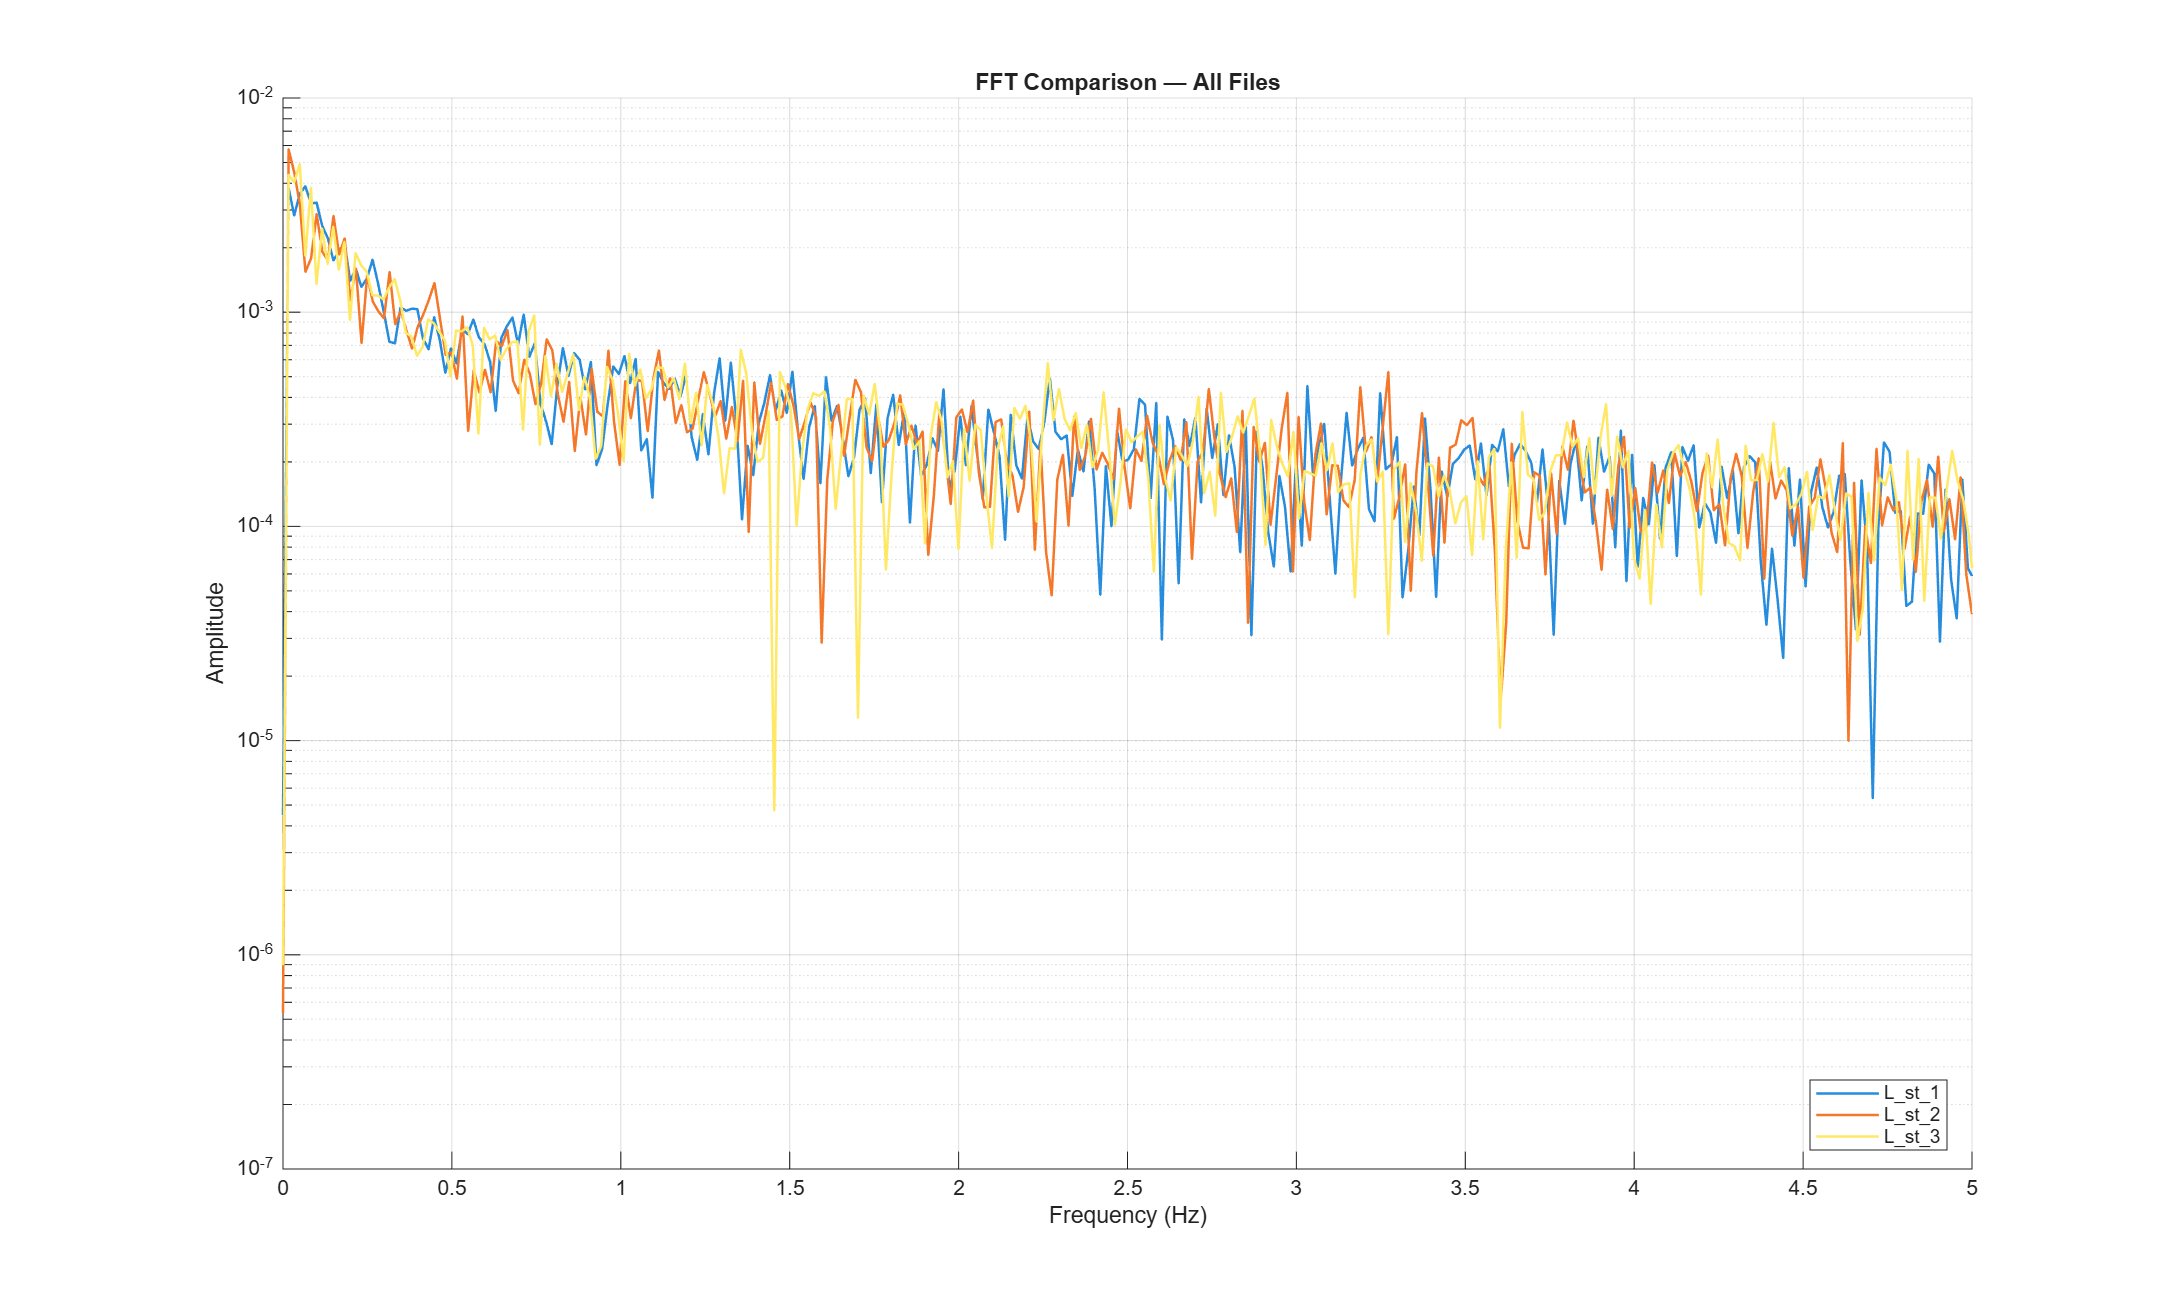
\includegraphics[width=\textwidth,height=7cm]{Figures/3_Still_Comparison.png}
		\caption{FFT plot for the 0.64 mm cable under stationary conditions.}
		\label{fig:still-c-064}
	\end{figure}
	
	\clearpage
	\subsection{Moving Conditions}
	
	\vspace{1cm}
	
	\begin{figure}[htbp]
		\centering
		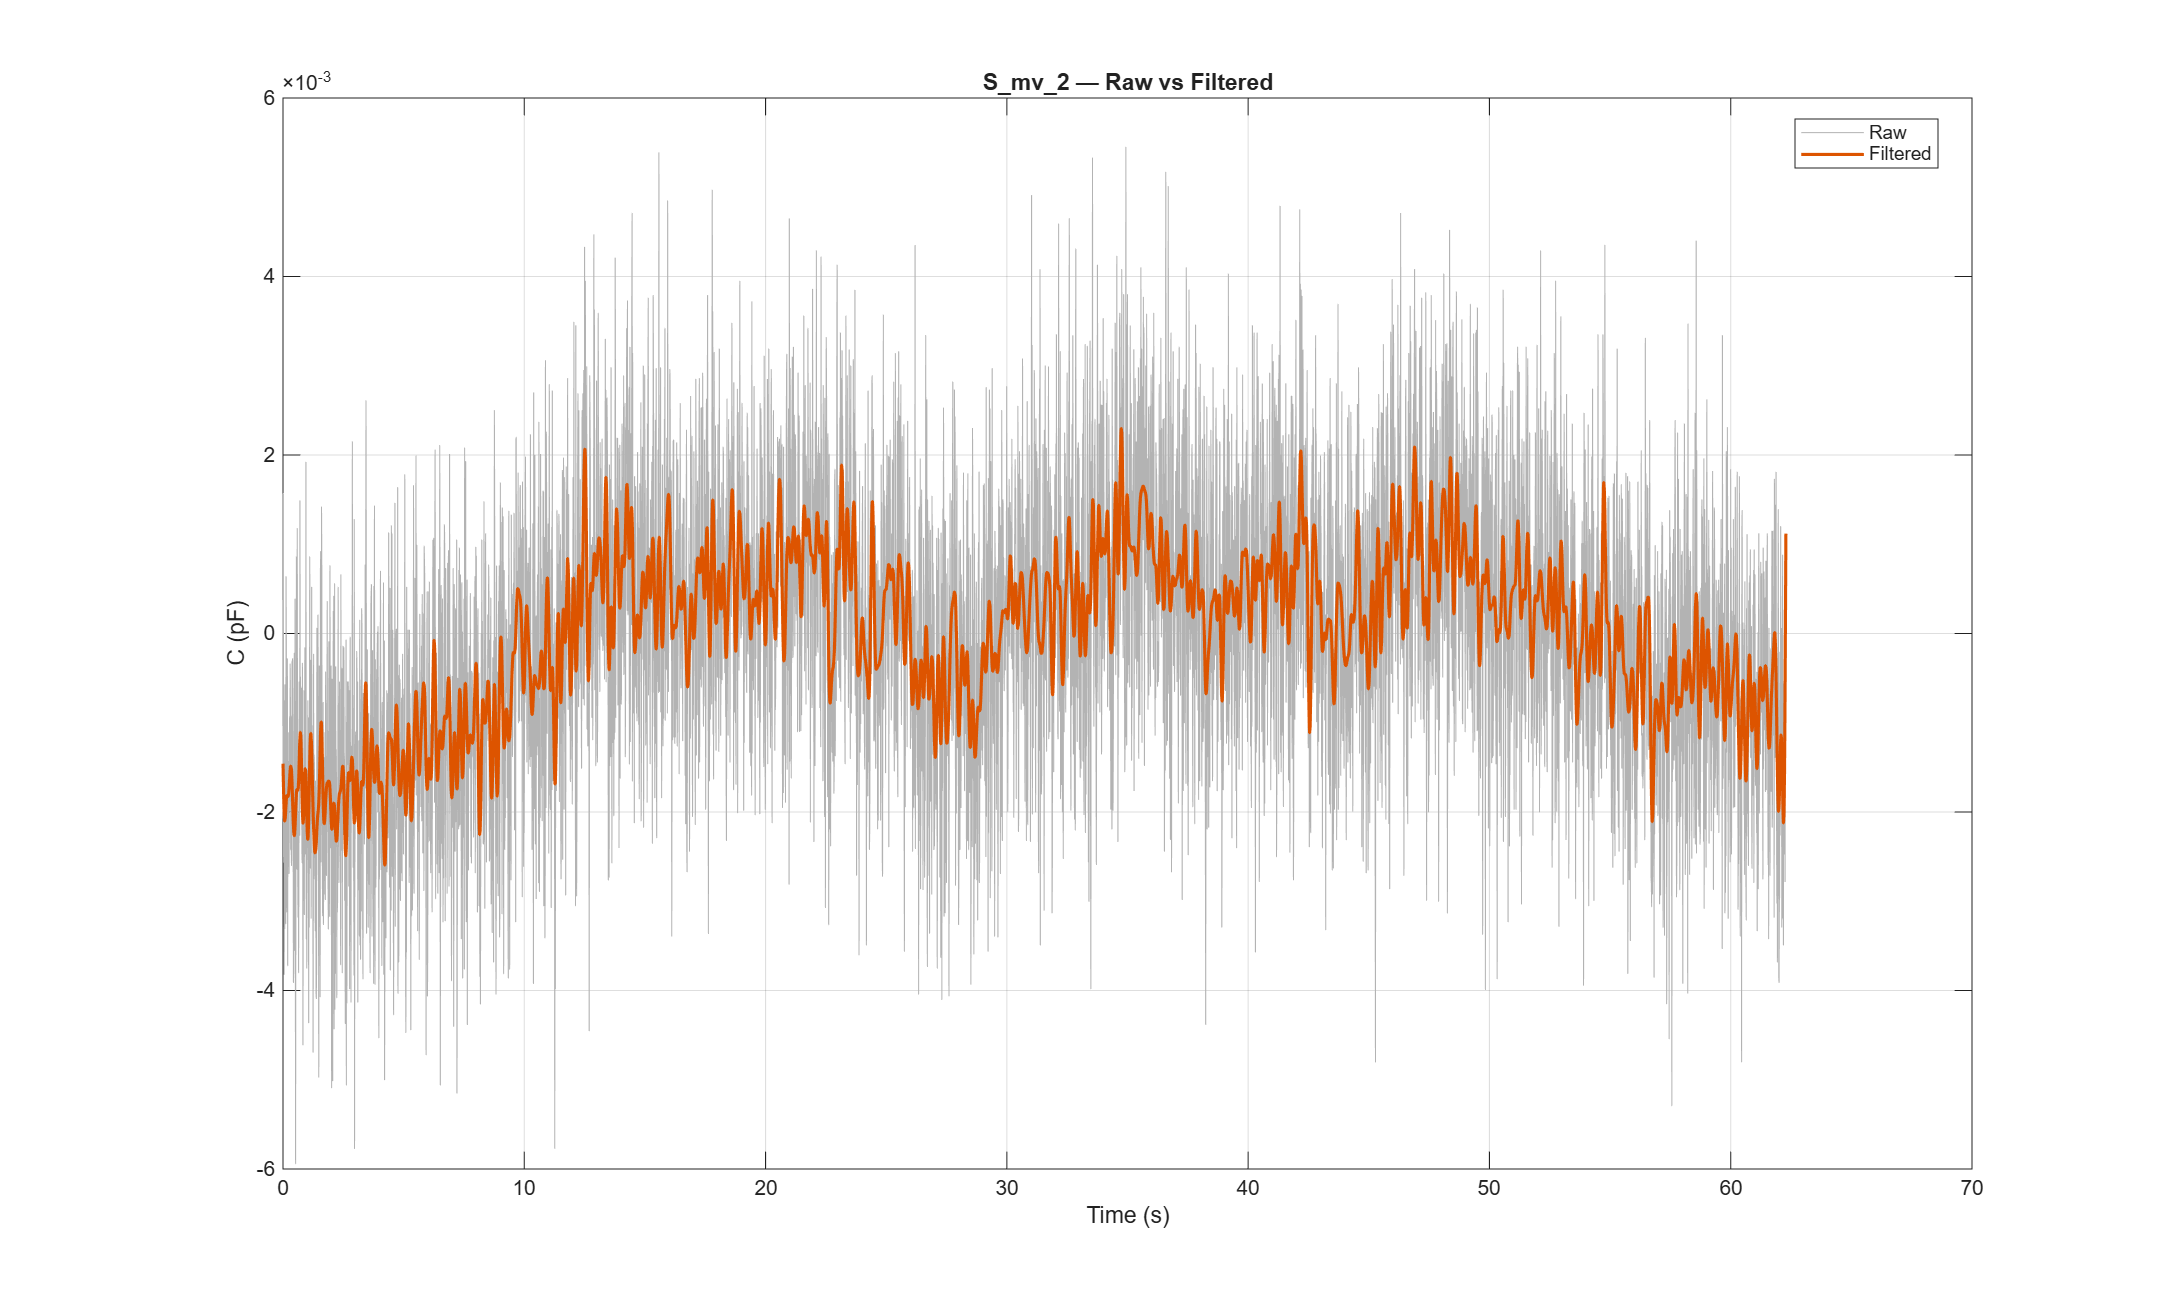
\includegraphics[width=\textwidth,height=7cm]{Figures/1_Moving_filtered.png}
		\caption{Filtered capacitance measurements for the 0.32 mm cable under moving conditions.}
		\label{fig:moving-f-032}
	\end{figure}
	
	\vspace{1cm}
	
	\begin{figure}[htbp]
		\centering
		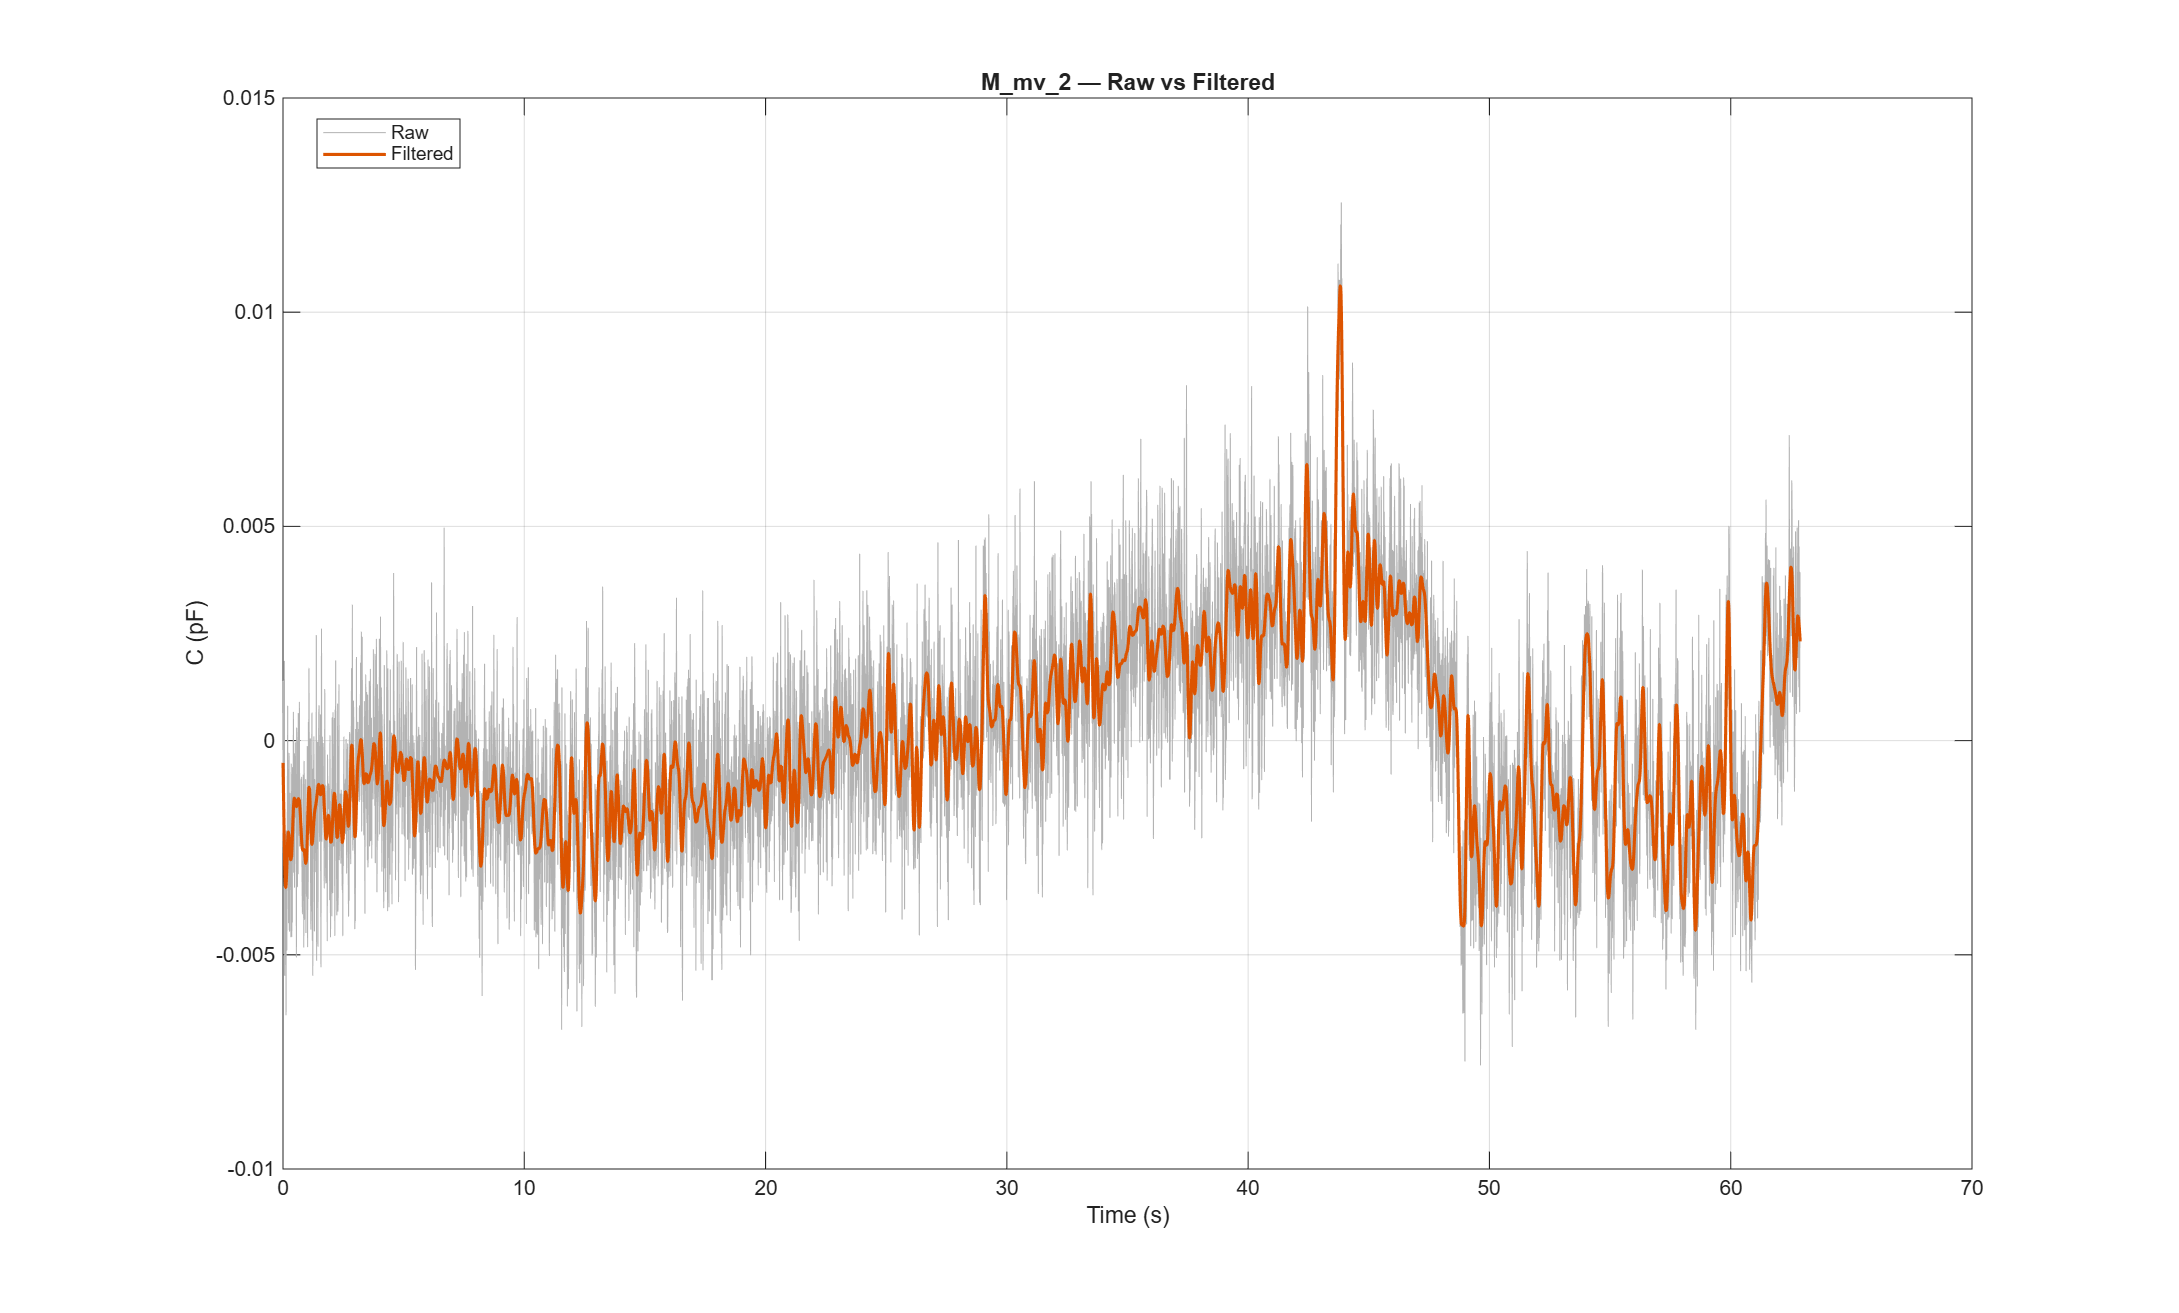
\includegraphics[width=\textwidth,height=7cm]{Figures/2_Moving_filtered.png}
		\caption{Filtered capacitance measurements for the 0.40 mm cable under moving conditions.}
		\label{fig:moving-f-040}
	\end{figure}
	
	\begin{figure}[htbp]
		\centering
		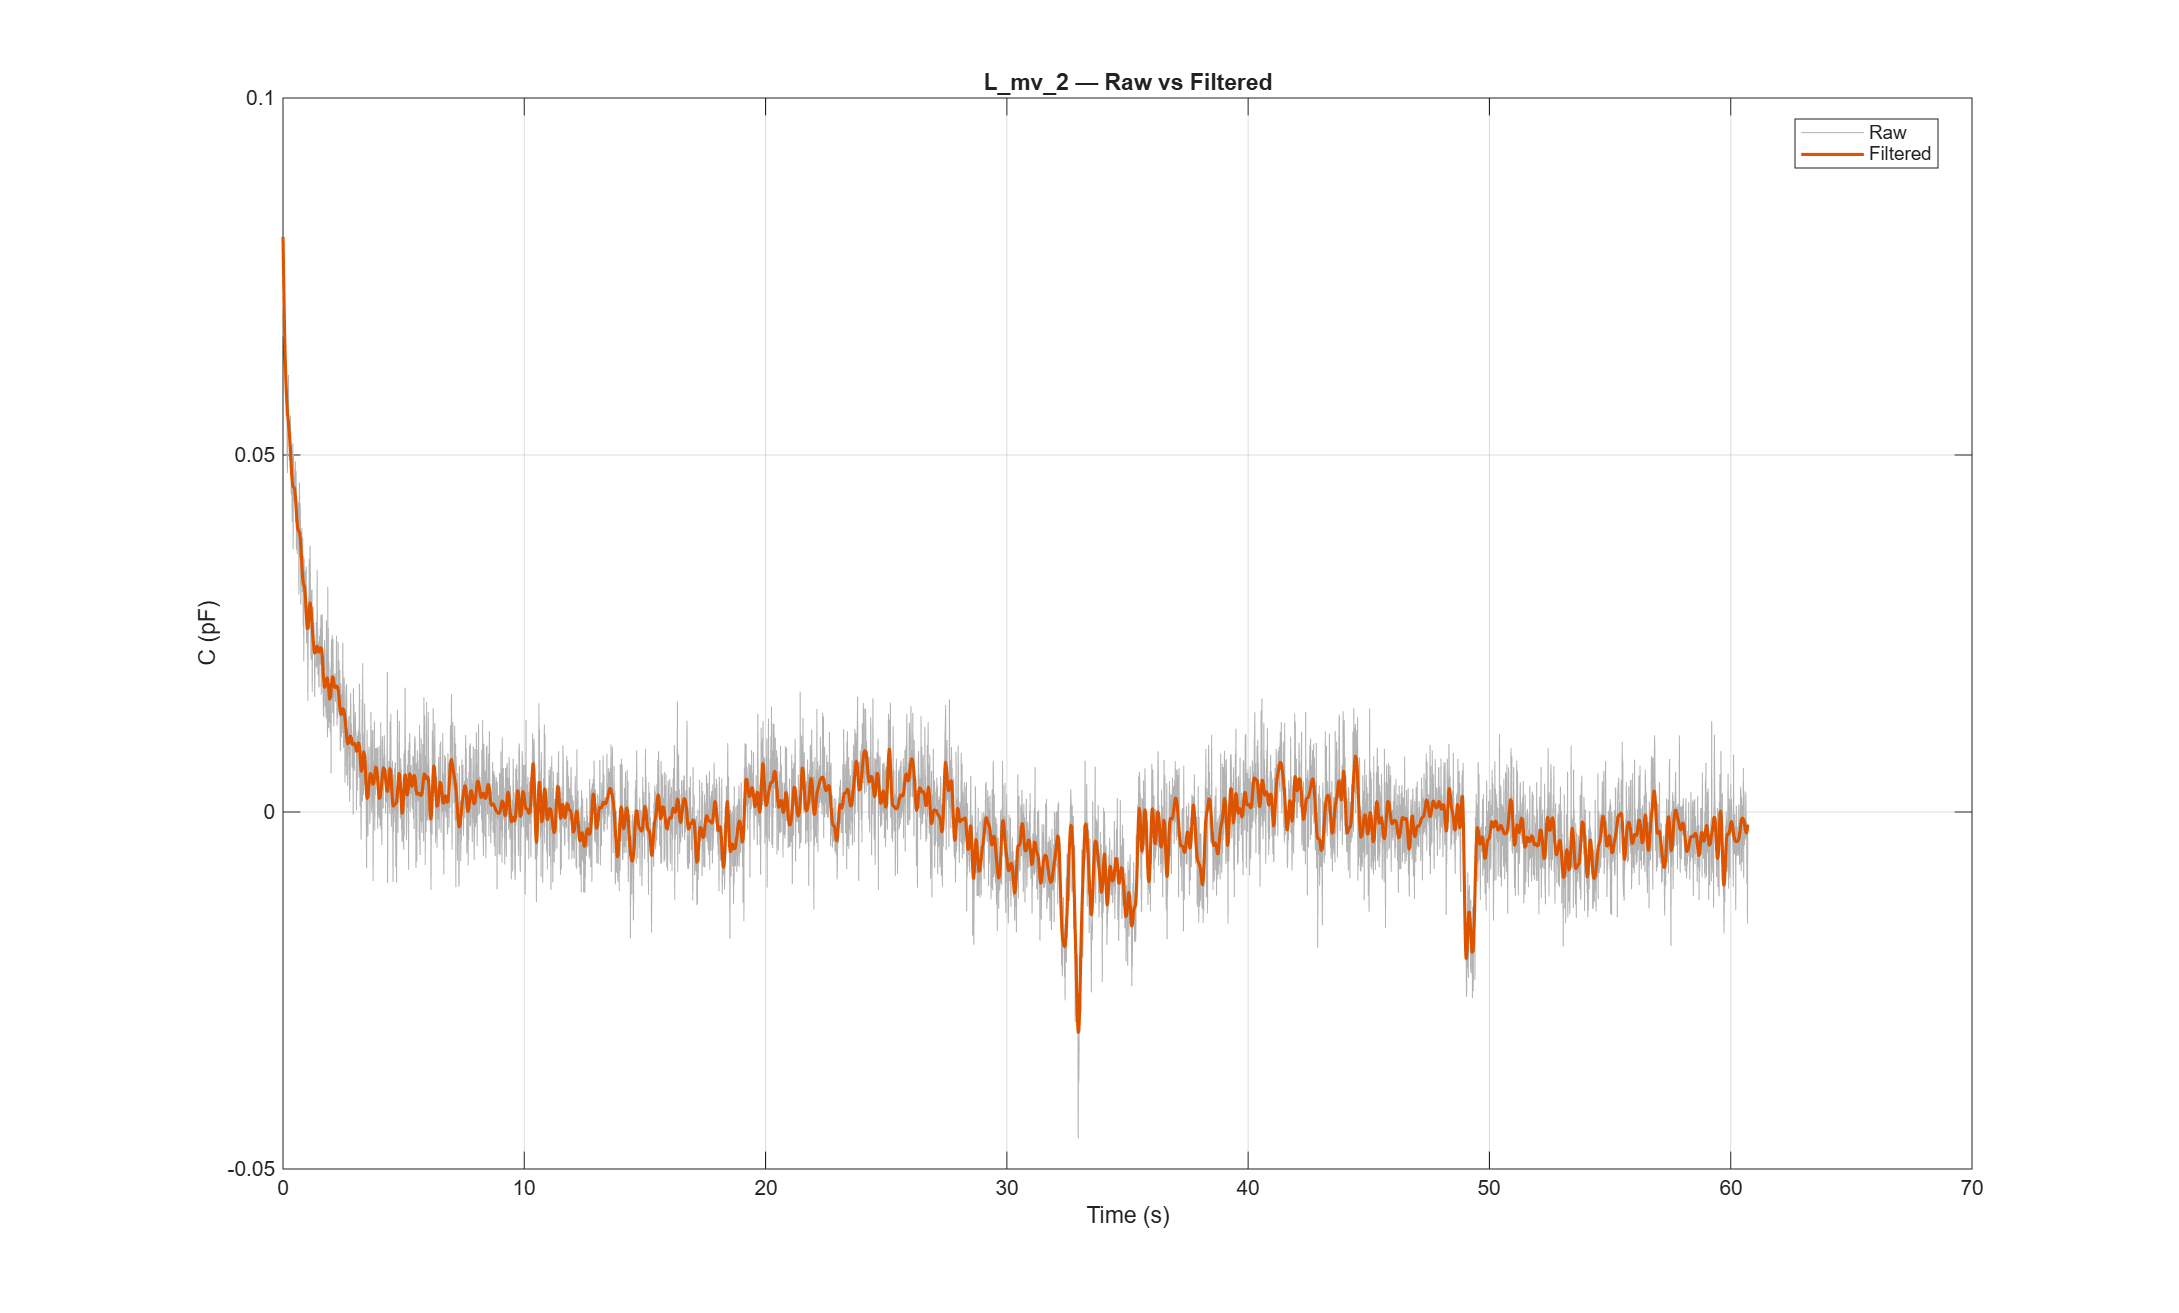
\includegraphics[width=\textwidth,height=7cm]{Figures/3_Moving_filtered.png}
		\caption{Filtered capacitance measurements for the 0.64 mm cable under moving conditions.}
		\label{fig:moving-f-064}
	\end{figure}
	
	\begin{figure}[htbp]
		\centering
		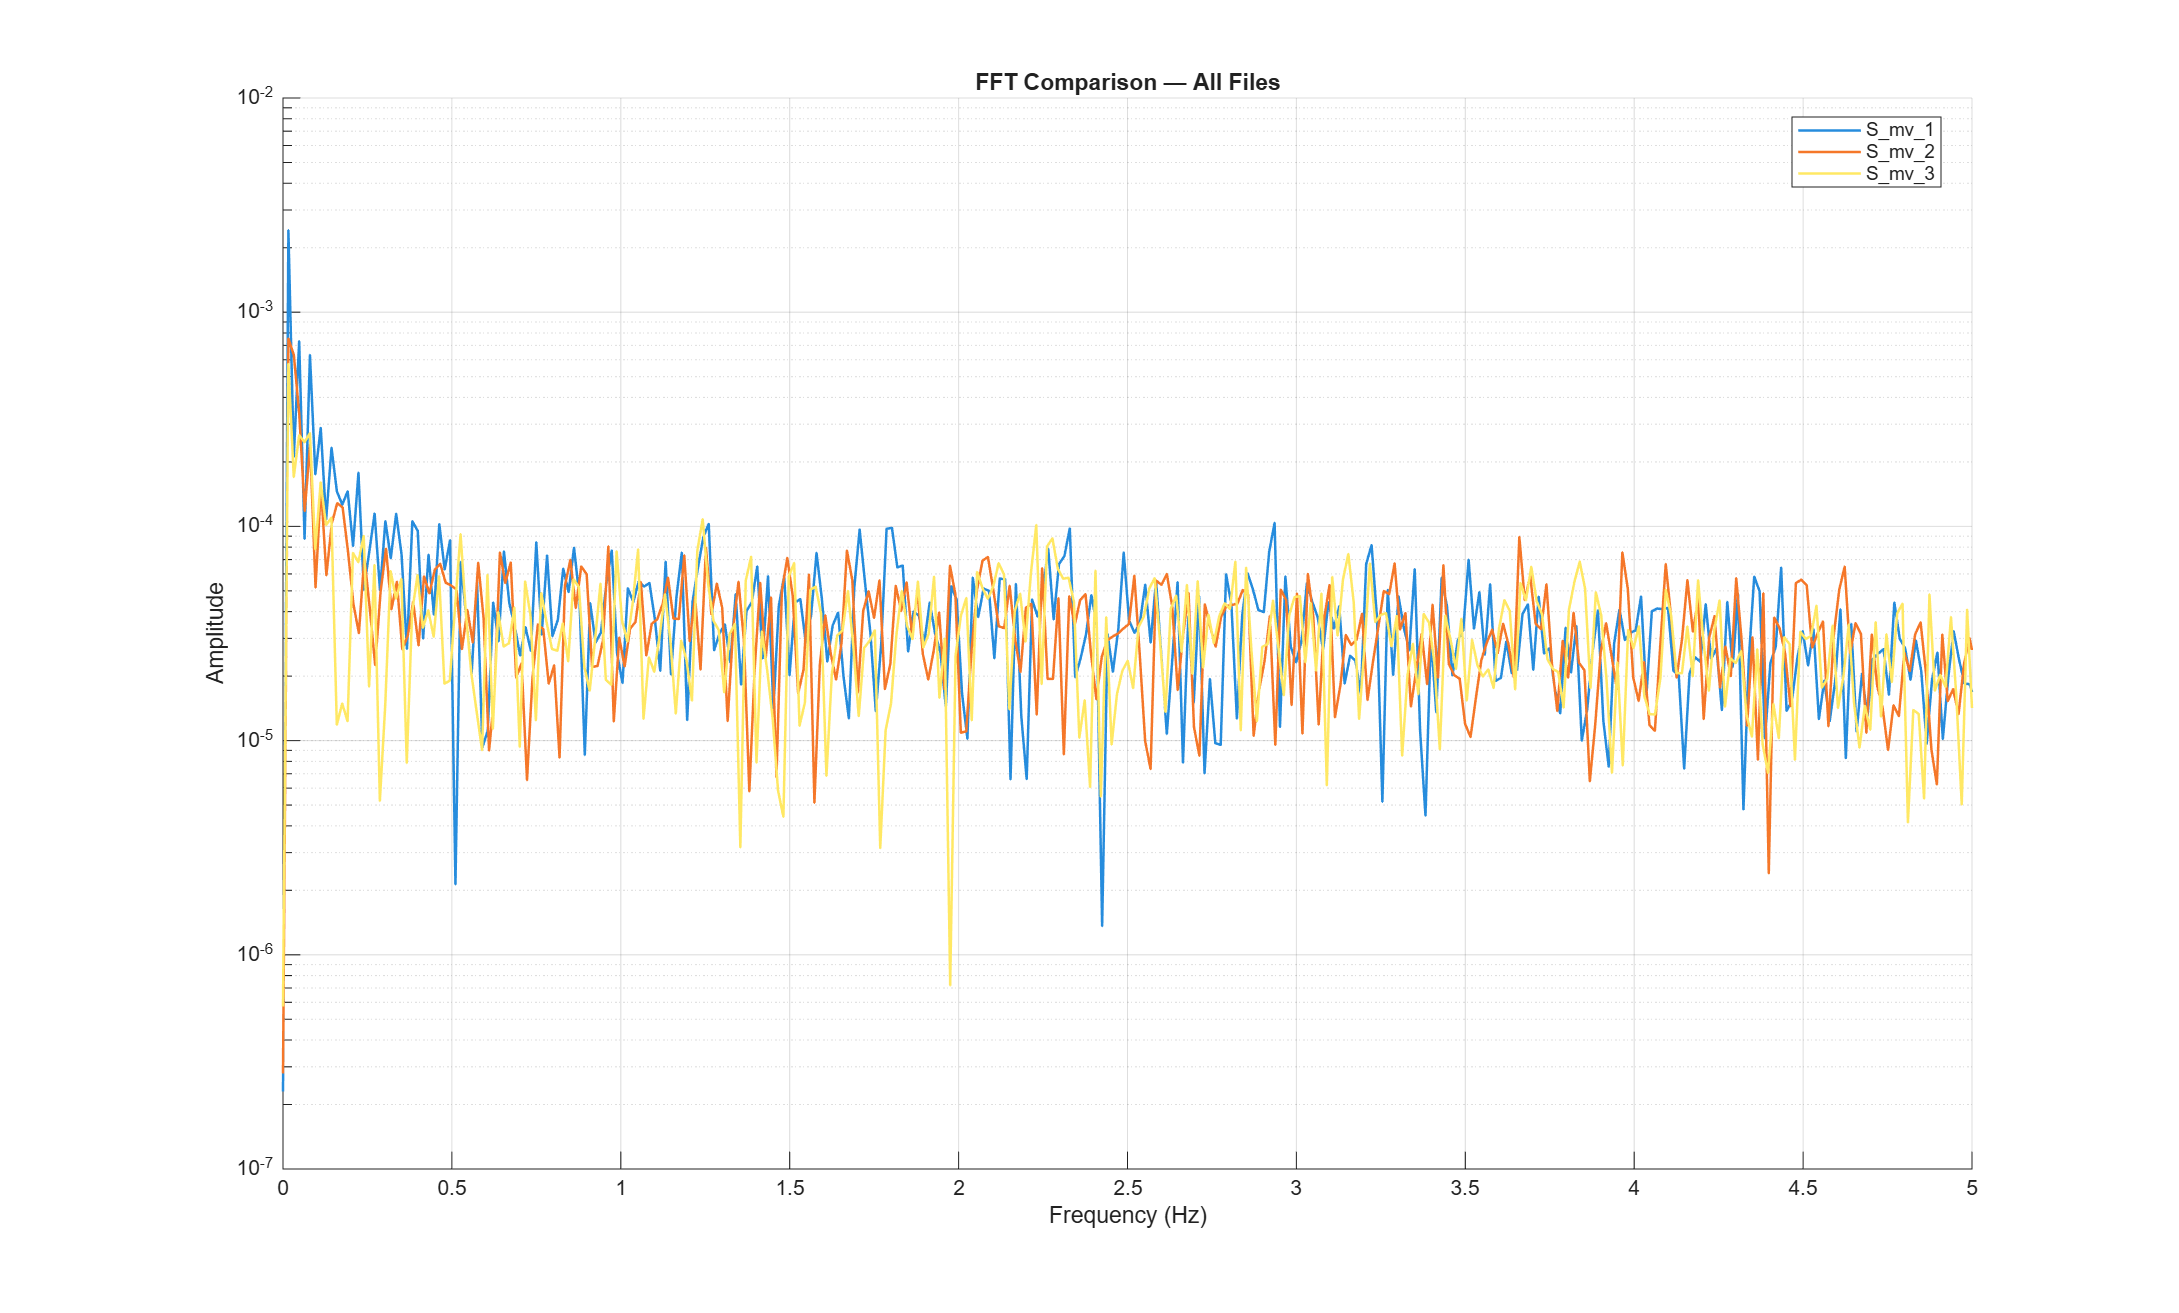
\includegraphics[width=\textwidth,height=7cm]{Figures/1_Moving_Comparison.png}
		\caption{FFT plot for the 0.32 mm cable under moving conditions.}
		\label{fig:moving-c-032}
	\end{figure}
	
	\begin{figure}[htbp]
		\centering
		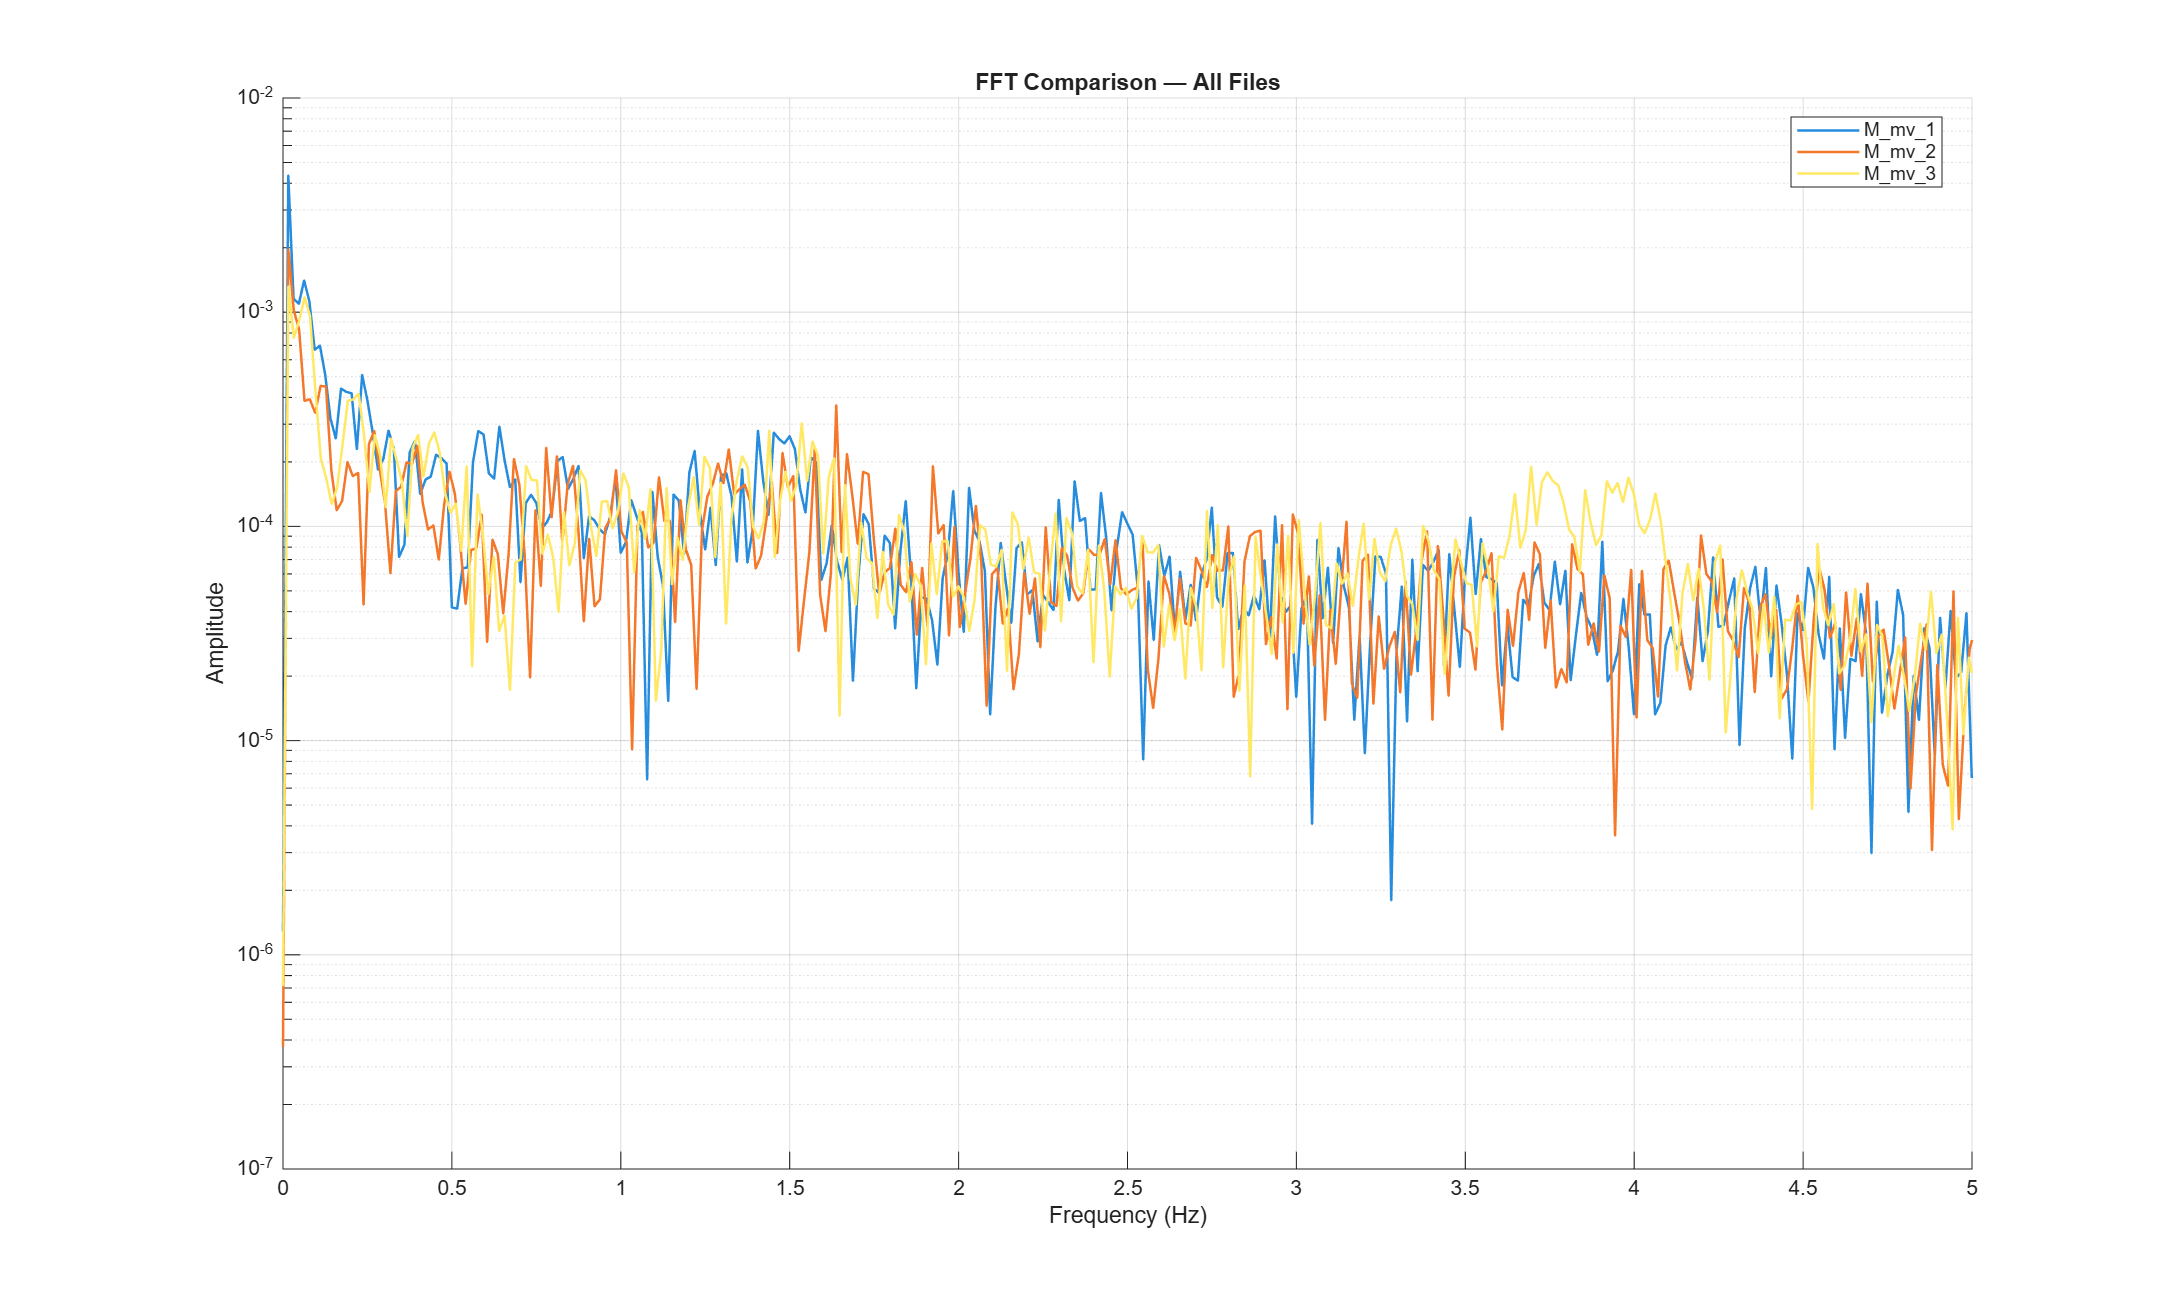
\includegraphics[width=\textwidth,height=7cm]{Figures/2_Moving_Comparison.png}
		\caption{FFT plot for the 0.40 mm cable under moving conditions.}
		\label{fig:moving-c-040}
	\end{figure}
	
	\begin{figure}[htbp]
		\centering
		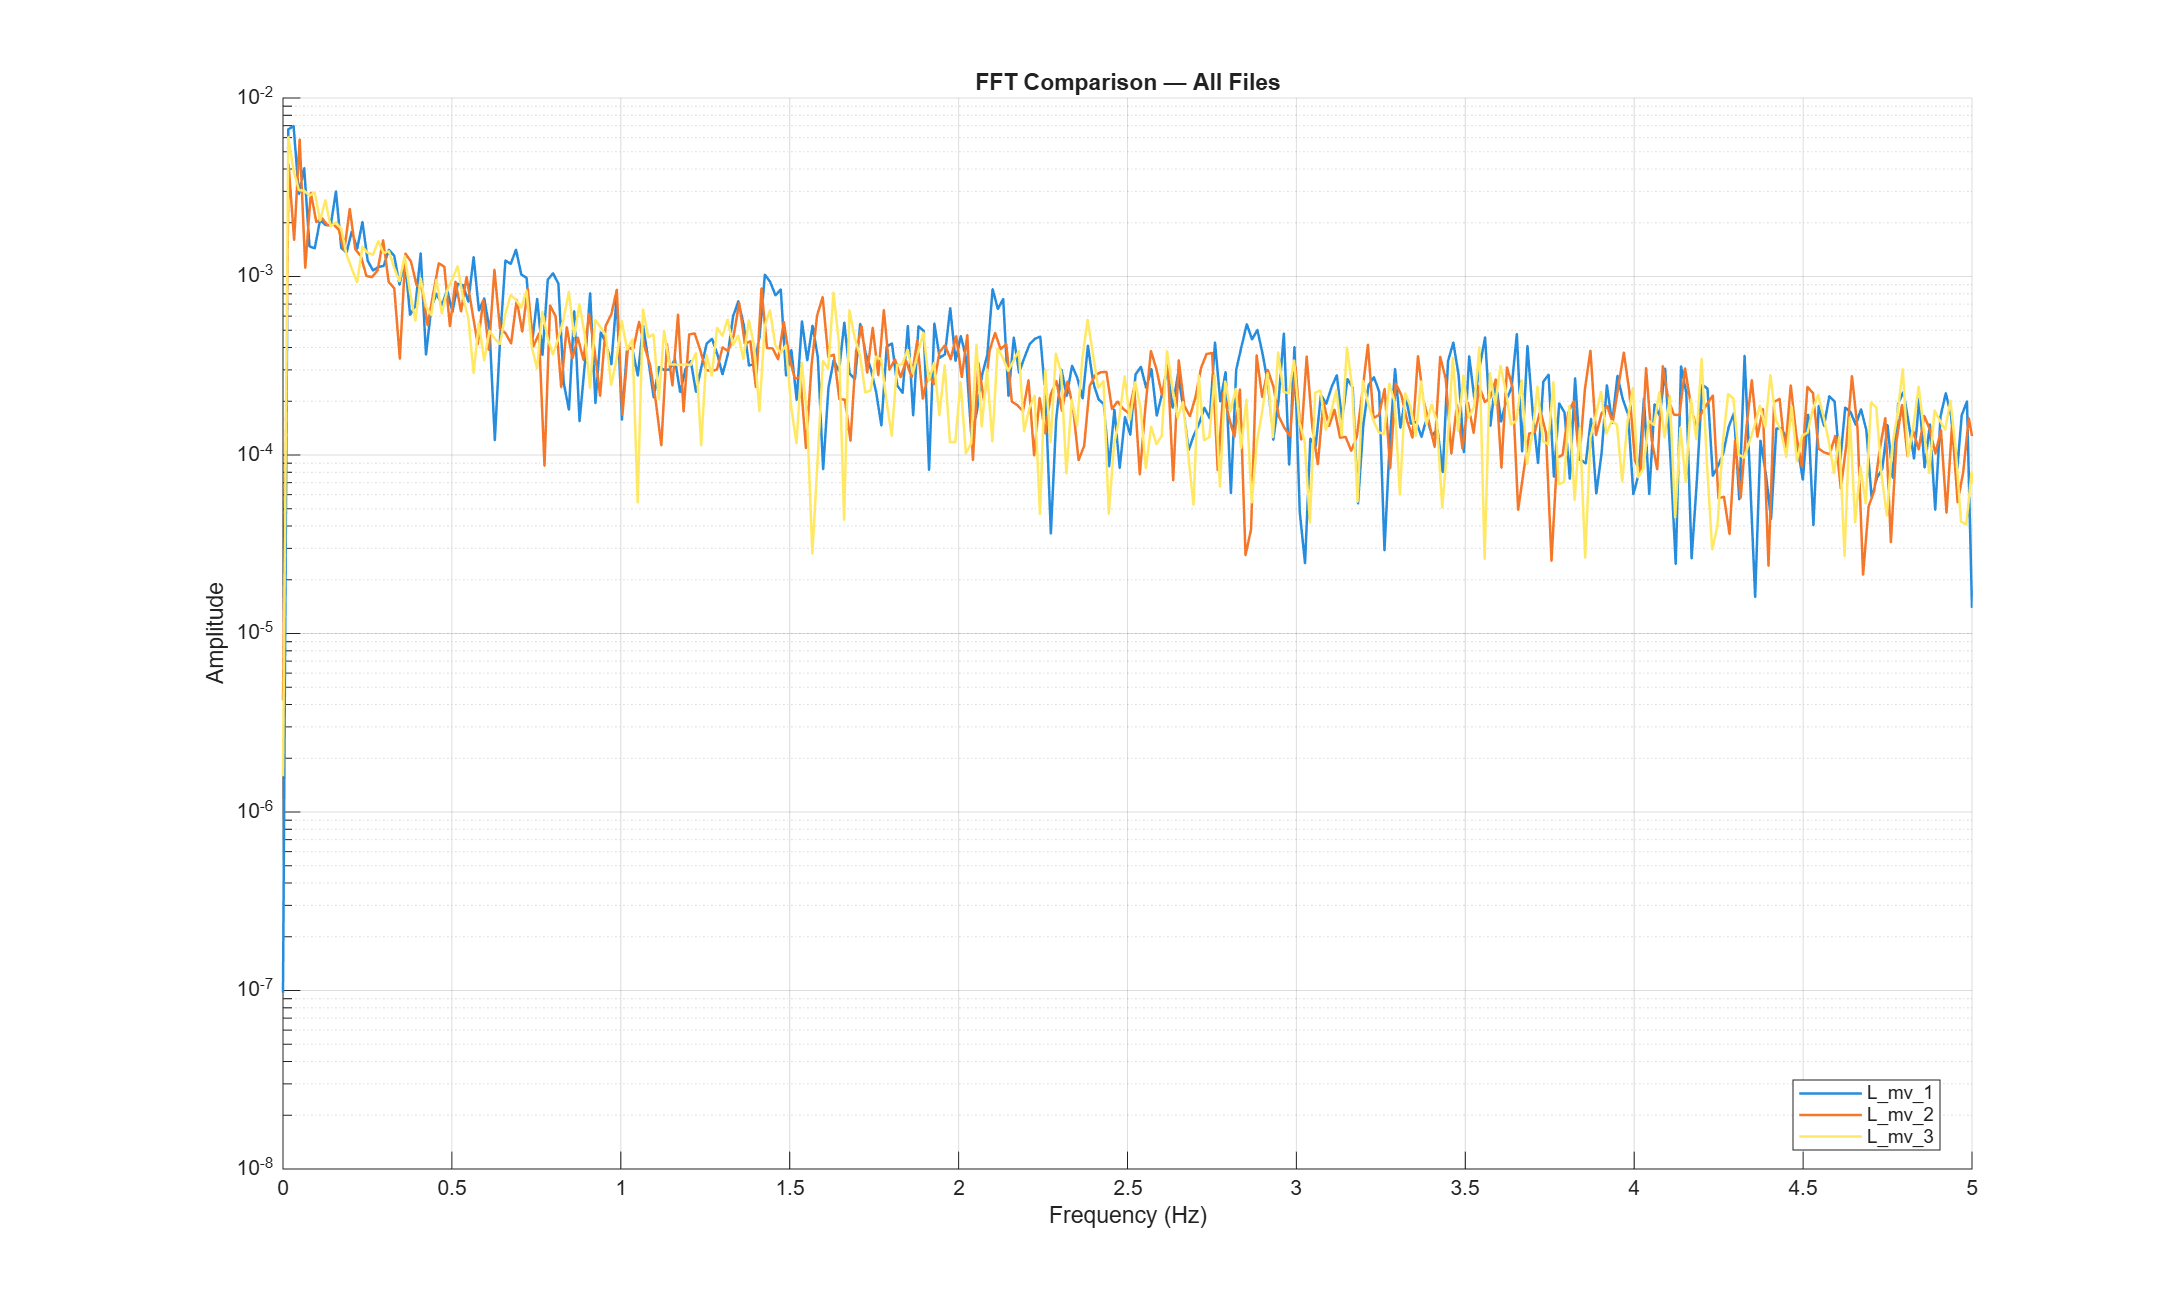
\includegraphics[width=\textwidth,height=7cm]{Figures/3_Moving_Comparison.png}
		\caption{FFT plot for the 0.64 mm cable under moving conditions.}
		\label{fig:moving-c-064}
	\end{figure}
	
\end{document}